\documentclass[11pt]{article}
\usepackage{amsmath,amssymb,amsthm}
\usepackage[margin=1in]{geometry}
\usepackage{booktabs}
\usepackage{graphicx}
\graphicspath{{../figures/}}
\usepackage[hidelinks]{hyperref}
\newtheorem{lemma}{Lemma}
\newtheorem{proposition}[lemma]{Proposition}
\newtheorem{corollary}[lemma]{Corollary}
\theoremstyle{remark}
\newtheorem{remark}[lemma]{Remark}
\newcommand{\E}{\mathbb{E}}
\newcommand{\Prob}{\mathbb{P}}
\newcommand{\1}{\mathbf{1}}
\newcommand{\pending}[1]{\par\medskip\noindent\fbox{\parbox{\dimexpr\linewidth-2\fboxsep-2\fboxrule}{\small\sffamily
Draft, results pending: #1}}\par\medskip}
\hypersetup{pdftitle={Fitting and choosing radiative-transfer emulators for the retrieval},pdfauthor={Yitzchak Shmalo}}

\title{Fitting and choosing radiative-transfer emulators for the retrieval}
\author{Yitzchak Shmalo\thanks{Einstein Institute of Mathematics, The Hebrew University of Jerusalem, Jerusalem,
Israel. \texttt{yitzchak.shmalo@gmail.com}.}}
\date{}

\begin{document}
\maketitle

\begin{abstract}
Radiative-transfer emulators are fitted to a code's outputs but used through an inverse, the retrieval of surface
reflectance. We give the retrieval error exactly in terms of the component errors and show that the forward and
retrieval rankings of two emulators differ by a change of measure with density proportional to $t^2/q^4$. Training on
the retrieval error is regression under a known, unbounded covariate shift whose price in effective sample size can be
computed before any training. On the EMIT table, networks trained on the square root of the retrieval weights floored
at a hundredth of the median transmission lower the radiance error by $8\%$ and the 95th percentiles of the retrieval
error by $32$ to $44\%$ on every one of ten splits. On the libRadtran benchmark of Mazid and Rishe the same weights
lower the radiance error from $0.81\%$ to $0.17\%$ and the retrieval tail from $3.2$ to $0.5$ points on every seed, at
a larger error in the spherical albedo. Two failed evaluations of the code in the EMIT table make every weighted network
worse than the plain one, and refitting a convex stack on the retrieval error lowers its tail by a quarter.
\end{abstract}

\section{Introduction}

At each band the top-of-atmosphere radiance over a Lambertian surface of reflectance $\rho$ is
\[
L(\rho)=a+\frac{\rho t}{1-\rho s},
\]
with path radiance $a$, transmission $t$ and spherical albedo $s$, and atmospheric correction recovers $\rho$ from a
measured radiance by inverting this relation \cite{isofit}. Computing $(a,t,s)$ with a radiative-transfer code such as
MODTRAN \cite{modtran}, libRadtran \cite{mayer,emde} or 6S \cite{vermote} for every pixel is too slow, and the codes
are replaced by emulators fitted to tables of their outputs \cite{brodrick,vicentservera}. The emulators are fitted and
compared by their forward error, the error in the emulated components or in the radiance they produce, but they are
used through the inverse. An error in the emulated components enters the retrieved reflectance divided by the slope
$\partial_\rho L=t/q^2$, $q=1-\rho s$, so that the same forward error costs little where the transmission is large and
a great deal where it is small. On tables that reach into strong absorption the two criteria can rank emulators
differently: on the EMIT atmospheric-correction table a convex stack of kernel and network emulators has the lowest
radiance error of the emulators compared and a larger tail of the retrieval error than the best of its members
\cite{shmalo2}.

The question here is what an emulator should be fitted to, and chosen by, when it is used through an inverse. The
answer has three parts.

The retrieval error has an exact closed form in the three component errors (Lemma~\ref{lem:exact}). To first order it
is the forward error at $\rho$ divided by the slope, and over a range of reflectances it is a Mahalanobis norm of the
component errors with a metric that depends on the state only through $(t,s)$ and is positive definite once three
reflectances are used (Proposition~\ref{prop:rank}). The forward and retrieval rankings of two emulators differ by a
change of measure with density proportional to $t^2/q^4$ (Proposition~\ref{prop:measure}), and on the EMIT table the
convex stack's net excess of squared retrieval error lies in the tenth of the entries where that density is smallest.

Training on the retrieval error is regression under a covariate shift whose likelihood ratio is known in closed form
and is unbounded as $t\to0$; a floor on $t$ truncates it as in the reweighted estimators of \cite{mpw}. The rate that a
fit certified in the weighted norm guarantees is sharp (Propositions~\ref{prop:weighted-rate}
and~\ref{prop:weighted-attained}), and the price of the weighting can be computed before any training: the effective
sample size of the floored weights is of the order of the number of entries below the floor
(Proposition~\ref{prop:neff}), and a fraction $(2-\beta)/2$ of their weight lies below the floor
(Corollary~\ref{cor:below}). On the EMIT table that weight sits in about thirty of the 285 bands, those of the
water-vapour absorption, and it keeps most of the states. Networks trained on the weighted objective show the price
from both sides (Section~\ref{sec:networks}). On the EMIT table the floored weights at a tenth of the median
transmission lower the tail of the retrieval error on the physical domain on every split, by nearly a quarter to more
than a third on average, and leave the radiance error unchanged, and a rule fixed before the runs, which chooses the floor on the validation block,
picks that floor on every split. At lower floors, which keep fewer effective entries, the weighted objective still
falls but the radiance error grows, and at the lowest floor every tail with it; the objective at a low floor is
attained best on held-out states by the fit one decade above it. Flattening the weights, $\bar w_\tau^{\,\kappa}$ with
$0<\kappa<1$ \cite{shimodaira}, does better than any floor: at a hundredth of the median transmission and $\kappa=1/2$
the network lowers the radiance error by $8\%$ and the four tails by $32$ to $44\%$ on average, each on every split,
and it attains the floored objectives on held-out states better than the networks fitted on them; only the albedo
error grows, by less than half. Kernel ridge regression fitted on the floored weights, the truncated reweighting of
\cite{mpw}, repeats the pattern of the floors (Section~\ref{sec:kernelfit}): at a tenth of the median transmission it
lowers every physical tail on every split, by $9$ to $15\%$, at $12\%$ more radiance error, and at a thousandth its
objective on held-out states falls to $0.08$ of the plain fit's while the radiance error and two of the tails rise. The table holds two failed evaluations of the code, with zero transmission in most bands. A floored weight
gives such an entry the weight of $u^{-2}$ ordinary ones, and with the two in the table every weighted network is worse
on held-out states than the plain one, on nearly every split even on the weighted objective itself. On a libRadtran table, where the floored
weights fall on one band of thirteen, no floor improves on the plain network in both the radiance error and the tails,
and the same rule picks one that is worse in the radiance error and in the physical tails. On the published benchmark
of \cite{pkan}, the same corpus split by its release into $35{,}000$ training states, with the 6S coefficients as an
input and the band as one, the flattened and floored weights lower the radiance error by factors of $3.6$ to $4.8$ and
every retrieval tail by factors of $5.3$ to $6.7$ on every seed; in the release's own metrics they cut the mean absolute
error to $0.37$ to $0.45$ of its best model's and raise the root-mean-square error by about a quarter, all of it from
the spherical albedo (Section~\ref{sec:pkan}).

Choosing a few numbers on the retrieval error is a different matter. The price of choosing among $K$ candidates on a
weighted criterion is set by the effective number of states rather than of entries (Proposition~\ref{prop:select}),
and the retrieval weights keep three quarters of the validation states or more. Refitting the weights of the convex
stack on the first-order retrieval error, with the members fitted on the forward error, lowers the 95th percentile of
the retrieval error on the physical domain below that of the component stack on 39 of 40 held-out halves of the EMIT
table, by a quarter at the median, to the level of the kernel on learned features, the best single member
(Section~\ref{sec:stacks}); every stack that no other improves on both counts minimizes one of a one-parameter family
of mixed objectives (Proposition~\ref{prop:pareto}). Chosen on the cut criterion, the input length scales of a kernel
regression move toward the water-vapour column and nearly halve its tail on the physical domain, at four and a half
times its radiance error; at that radiance error, about the networks' own, the tail is a fifth of the plain network's
(Section~\ref{sec:kernels}). The stopping epoch of a network, a choice among many close candidates, has
little to give either way (Section~\ref{sec:epochs}).

\paragraph{Outline.} Section~\ref{sec:related} reviews related work. Section~\ref{sec:exact} gives the retrieval error
and its metric, Section~\ref{sec:measure} the change of measure, Section~\ref{sec:training} what a weighted fit
guarantees and what it costs, and Section~\ref{sec:choosing} the price of choosing on a weighted criterion and the
family of stacking objectives. Section~\ref{sec:data} describes the tables, the emulators and the scores, and
Section~\ref{sec:experiments} the experiments.

\section{Related work}\label{sec:related}

\paragraph{Radiative transfer and its inversion.} The relation $L=a+\rho t/(1-\rho s)$ for a Lambertian surface goes
back to the modelling of satellite measurements of ground reflectance in \cite{tanre1979}. Operational atmospheric
correction evaluates it with a radiative-transfer code, 6S and its vector version \cite{vermote,kotchenova2006},
libRadtran \cite{mayer,emde} or MODTRAN \cite{modtran}, directly or through lookup tables, as in ATCOR
\cite{richter2002} and in the algorithms reviewed in \cite{gao2009}. For imaging spectroscopy the retrieval is posed as
optimal estimation \cite{rodgers}: ISOFIT inverts the surface and the atmosphere jointly for EMIT \cite{isofit}, and the
uncertainty of the retrieved reflectance is quantified in \cite{thompson2020}. The carbon-dioxide retrievals of OCO-2
invert a full-physics forward model in the same framework \cite{connor,odell,crisp,eldering}, and fast
principal-component approximations of the radiative transfer \cite{kopparla2016} have been judged by the errors they
cause in these retrievals \cite{somkuti2017,somkuti2020}. The benchmark of Section~\ref{sec:pkan} uses the thirteen bands of
Sentinel-2 \cite{drusch2012}.

\paragraph{Emulators of radiative transfer.} Networks have replaced parts of atmospheric models since the emulation of
longwave radiation in a climate model \cite{krasnopolsky}, and more recently for gas optics and for the whole transfer
calculation \cite{veerman,ukkonen}. Learned parameterizations of subgrid processes \cite{rasp} are fitted offline and
used inside the model, and accuracy offline does not guarantee a stable coupled simulation \cite{brenowitz}, a
counterpart of the gap between forward and retrieval error studied here. In remote sensing, statistical emulators of radiative-transfer models are surveyed in
\cite{verrelst2025}, packaged in the toolbox of \cite{rivera}, used for global sensitivity analysis \cite{verrelst2015}
and built on Gaussian processes \cite{gomezdans,campsvalls}. The sRTMnet emulator corrects a fast approximation toward
MODTRAN inside ISOFIT \cite{brodrick}; Vicent Servera et al.\ \cite{vicentservera} compare regression emulators of the
MODTRAN transfer functions and evaluate the corrected reflectance; Lamminp\"a\"a et al.\ \cite{lamminpaa} fit a
Gaussian-process emulator of the OCO-2 forward model by cross-validated forward error and use its analytic Jacobians in
the retrieval. Surrogates of radiative transfer also serve inversions of exoplanet atmospheres \cite{himes2022},
atmospheric sounding \cite{sgattoni2024} and, for atmospheric transport, greenhouse-gas flux inversions
\cite{dadheech2025}. The correction of a cheap code toward an expensive one is multi-fidelity modelling
\cite{kennedyohagan,perdikaris,peherstorfer} in the tradition of the design and analysis of computer experiments
\cite{sacks}; the pKANrtm emulator of \cite{pkan} fits the libRadtran residual of 6S with a Kolmogorov--Arnold network
\cite{kan,kolmogorov}. The emulators compared in \cite{shmalo2} and used here are networks, Mat\'ern kernel regressions
\cite{stein,rw} and their combinations. None of these fits is weighted by the retrieval.

\paragraph{Surrogates for inverse problems.} In Bayesian inverse problems \cite{kaipiobook,stuart2010} the effect of a
surrogate on the solution has been treated as an approximation error in the likelihood \cite{kaipio}, bounded through
moments of the emulator error in the Hellinger distance between posteriors \cite{stuartteckentrup}, and controlled by an
$L^2$ error weighted by the posterior, which suggests where to place training points \cite{helin}. Surrogates refined
where the posterior concentrates \cite{limarzouk2014,cleary2021,gao2024uq}, corrected by the residual of the forward
model \cite{cao2023}, enriched with gradient information \cite{semler2024}, or fitted on a reduced parameter space
informed by the likelihood \cite{cui2014,cui2016,zahm2022} all aim the fit at the inverse problem; the propagation of
surrogate uncertainty into the posterior is studied in \cite{reiser2025}, and training data chosen to match the
information needed downstream in \cite{kurniawan2026}. Goal-oriented model reduction \cite{buithanh}, goal-oriented
inference \cite{lieberman2012,lieberman2014,spantini2017} and goal-oriented surrogates for stochastic inversion
\cite{mattis2018} fit the reduced model to the quantity of interest. Derivative-informed training fits a network to
the sensitivities as well as the values \cite{czarnecki,berguin2024}, and derivative-informed neural operators
\cite{oleary2022,oleary2024} accelerate Bayesian inversion \cite{cao2025}; \cite{behroozi} constrain the sensitivities
of a neural operator for forward and inverse modelling. The weight here comes from the retrieval equation in closed
form and acts on the three component errors jointly through a metric.

\paragraph{Training for the task.} Fitting a model by the loss of the decision it feeds is decision-focused learning
\cite{donti2017,wilder2019,mandi2024}, with the predict-then-optimize loss of \cite{elmachtoub2022}, its generalization
bounds \cite{elbalghiti2023}, learned surrogate losses \cite{shah2022} and decision-focused surrogate models in process
engineering \cite{gupta2024}. The retrieval is a decision of this kind, but its sensitivity to the emulator is known in
closed form, so the task loss is a weighted forward loss and needs no differentiation through a solver.

\paragraph{Covariate shift and weights.} Weighting by a known likelihood ratio is the classical answer to covariate
shift \cite{shimodaira,sugiyamabook,quionero2009}, with importance-weighted cross-validation \cite{sugiyama2007},
estimated ratios \cite{huang2007} and a learning theory of the correction \cite{cortes2008,cortes}. It is needed when
the model is misspecified and not when it is correctly specified \cite{shimodaira}; for nonparametric models that are
misspecified it is again needed for the best approximation under the target distribution \cite{gogolashvili}, and the
benefit of labels from the target depends on how singular the shift is \cite{kpotufe2021}. For kernel ridge regression
with an unbounded ratio of finite second moment the truncated reweighting of \cite{mpw} is minimax optimal, and in
general the estimation error of an importance-weighted fit is controlled by the second moment of the weights
\cite{cortes}. For overparameterized networks the effect of importance weights fades as training proceeds without
regularization \cite{byrdlipton}. Truncating weights \cite{ionides2008} and smoothing their tail \cite{psis} are the
importance-sampling counterparts of the floor and of the flattening used here, and the effective sample size of a
weighted average is Kish's \cite{kish}, discussed at length in \cite{elvira2022}.

\paragraph{Choosing models and combining them.} The kernel parameters of Section~\ref{sec:kernels} are chosen on a
criterion evaluated on held-out states; cross-validation \cite{stonecv,arlot} and its closed form for ridge regression
\cite{gcv} are the usual criteria, and kernel flows \cite{owhadiyoo,hamziowhadi} learn kernel parameters by how much
the kernel interpolant changes when half of the data are dropped. Stacking \cite{wolpert,breiman} descends from the combination of forecasts
\cite{batesgranger}. The networks are trained with Adam \cite{adam} and stopped on held-out data \cite{prechelt}, in
PyTorch \cite{pytorch}.

\section{The retrieval error of an emulator}\label{sec:exact}

An emulator predicts $(\hat a,\hat t,\hat s)=(a+e_a,t+e_t,s+e_s)$, and the retrieval inverts the predicted relation at
the true radiance,
\[
\hat\rho=\frac{L-\hat a}{\hat t+\hat s(L-\hat a)},\qquad L=L(\rho).
\]
Write $q=1-\rho s$, so that $\partial_\rho L=t/q^2$.

\begin{lemma}[exact form of the retrieval error]\label{lem:exact}
Put
\[
\ell=-\frac{q}{t}\,(q\,e_a+\rho\,e_t)-\rho^2 e_s,\qquad
\delta=\frac{q}{t}\,(e_t-s\,e_a)+\rho\,e_s-\frac{q}{t}\,e_a e_s .
\]
Whenever the predicted denominator is nonzero,
\[
\hat\rho-\rho=\frac{\ell+(\rho q/t)\,e_a e_s}{1+\delta}.
\]
\end{lemma}

\begin{proof}
Let $u=L-a=\rho t/q$ and $D=t+su=t/q$, so that $\rho=u/D$. The predicted denominator is
$\hat D=\hat t+\hat s(u-e_a)=D+e_t+u\,e_s-s\,e_a-e_ae_s$, and
\[
\hat\rho-\rho=\frac{u-e_a}{\hat D}-\frac{u}{D}=\frac{-e_aD-u(e_t+u\,e_s-s\,e_a)+u\,e_ae_s}{D\hat D}.
\]
Since $D-su=t$, the numerator equals $-t\,e_a-u\,e_t-u^2e_s+u\,e_ae_s$. Divide numerator and denominator by
$D^2=t^2/q^2$ and use $u/D=\rho$, $uq^2/t^2=\rho q/t$ and $\hat D/D=1+\delta$.
\end{proof}

\begin{corollary}[first order]\label{cor:first}
As the component errors tend to zero relative to $t$,
\[
\hat\rho-\rho=\ell+O\!\left(\frac{|e|^2}{t^2}\right),\qquad
\ell=-\frac{q^2}{t}\bigl(\hat L(\rho)-L(\rho)\bigr)+O\!\left(\frac{|e|^2}{t^2}\right),
\]
where $\hat L(\rho)=\hat a+\rho\hat t/(1-\rho\hat s)$ and $|e|=|e_a|+|e_t|+t|e_s|$. The retrieval error is the forward
error at $\rho$ divided by the slope $\partial_\rho L=t/q^2$.
\end{corollary}

\begin{proof}
The first statement is Lemma~\ref{lem:exact} with $|\delta|=O(|e|/t)$. For the second, the forward error is
$\hat L(\rho)-L(\rho)=e_a+\rho e_t/q+\rho^2 t e_s/q^2+O(|e|^2)$, and multiplying by $-q^2/t$ gives $\ell$.
\end{proof}

Let $\nu$ be a probability measure on the reflectances of interest in $(0,R]$, and write $e=(e_a,e_t,e_s)^\top$ and
\[
v_\rho=\left(\frac{q_\rho^2}{t},\ \frac{\rho q_\rho}{t},\ \rho^2\right)^{\!\top},\qquad
M(t,s)=\int v_\rho v_\rho^\top\,\nu(d\rho),\qquad q_\rho=1-\rho s .
\]
By Corollary~\ref{cor:first}, $\int(\hat\rho-\rho)^2\,\nu(d\rho)=e^\top M(t,s)\,e+O(|e|^3/t^3)$ at every entry, so the
first-order mean squared retrieval error of an emulator over an evaluation distribution is the mean of a Mahalanobis
norm of its component errors, with a metric that depends on the state and the band only through $(t,s)$.

\begin{proposition}[rank of the metric]\label{prop:rank}
If $\nu$ is a point mass, $M$ has rank one. If the support of $\nu$ contains at least three points, $M$ is positive
definite for every $t>0$ and $s\in[0,1)$.
\end{proposition}

\begin{proof}
A point mass gives $M=v_\rho v_\rho^\top$. In general $x^\top Mx=\int(v_\rho^\top x)^2\,\nu(d\rho)$, and
$v_\rho^\top x=p_x(\rho)$ with $p_x(\rho)=x_1(1-2s\rho+s^2\rho^2)/t+x_2(\rho-s\rho^2)/t+x_3\rho^2$, a polynomial of
degree at most two. Its coefficients in the basis $(1,\rho,\rho^2)$ are $(x_1/t,\,(x_2-2sx_1)/t,\,(s^2x_1-sx_2)/t+x_3)$,
a triangular invertible map of $x$, so $p_x\equiv0$ only for $x=0$. A nonzero polynomial of degree at most two
vanishes at no more than two points, hence $x^\top Mx>0$ for $x\neq0$ once $\nu$ charges three.
\end{proof}

\begin{remark}
At a single reflectance the retrieval sees one combination of the three component errors, $v_\rho^\top e$, and is
blind to the two directions orthogonal to $v_\rho$. For small $t$ the first two coordinates of $v_\rho$ scale as $1/t$
and the third does not, so path-radiance and transmission errors are weighted by $1/t^2$ and the albedo error by a
constant, in agreement with the transfer inequality $|\bar\rho-\rho|\le e_R/t$, $e_R=|e_a|+R|e_t|+R^2t|e_s|$, of
\cite{shmalo2}, where the albedo enters as $R^2t|e_s|/t=R^2|e_s|$.
\end{remark}

A comparison with the exact inverse on $10^5$ random states, with component errors of the order of the components
themselves, reproduces Lemma~\ref{lem:exact} to within $1.5\times10^{-12}$.

\section{Forward and retrieval rankings differ by a change of measure}\label{sec:measure}

Fix $\rho$ and write $d_f=v_\rho^\top e_f$ for an emulator $f$ with component errors $e_f$. By
Corollary~\ref{cor:first}, to first order the retrieval error is $\hat\rho_f-\rho=-d_f$ and the forward error is
$r_f=\hat L_f(\rho)-L(\rho)=(t/q^2)\,d_f$. Let $p$ be a distribution over the entries, a state and a band, with
$\E_p[d_f^2]<\infty$, and put $g=t^2/q^4$.

\begin{proposition}[change of measure]\label{prop:measure}
If $0<\E_p[g]<\infty$, then $\E_p[r_f^2]=\E_p[g]\,\E_{p_g}[d_f^2]$ with $dp_g/dp=g/\E_p[g]$. Two emulators $f,h$ are
ordered by the forward squared error as they are ordered by the squared retrieval error under $p_g$. The orders under
$p$ and $p_g$ disagree, $\E_p[r_f^2]<\E_p[r_h^2]$ while $\E_p[d_f^2]>\E_p[d_h^2]$, exactly when $\Delta=d_f^2-d_h^2$
satisfies
\[
\E_p[\Delta]>0\quad\text{and}\quad \mathrm{Cov}_p(g,\Delta)<-\E_p[g]\,\E_p[\Delta].
\]
\end{proposition}

\begin{proof}
The first identity is $r_f^2=g\,d_f^2$ integrated against $p$. The second statement follows from
$\E_p[g\Delta]=\E_p[g]\E_p[\Delta]+\mathrm{Cov}_p(g,\Delta)$.
\end{proof}

Relative to the retrieval, the forward metric gives an entry of transmission $t$ a weight of order $t^2$. On the EMIT
table, where the transmissions of the physical domain range over more than twenty orders of magnitude, the forward
metric is blind to the entries that set the tail of the retrieval error, and an emulator whose excess squared error
sits at small transmission can win on the forward metric and lose on the retrieval. For the convex stack and the kernel
on learned features of \cite{shmalo2}, on three splits at two network widths and on the physical domain above
$10^{-3}T_{\rm train}$, the first-order forward error at $\rho=0.7$ favors the stack in all six runs, while the
first-order retrieval error favors the kernel on features by factors of $5.0$ to $9.9$ and the exact constrained
retrieval by factors of $3.3$ to $4.5$. The identity of Proposition~\ref{prop:measure} closes to rounding, and all of
the stack's net excess $\sum\Delta$ lies in the tenth of the entries with the smallest $g$. The Pearson correlation of
$g$ and $\Delta$ is only $-0.014$, because $\Delta$ is heavy-tailed; the covariance, not the correlation, is the
quantity the proposition needs.

\section{What a fit for the retrieval guarantees and what it costs}\label{sec:training}

Consider one output coordinate $c\in\{a,t,s\}$ at one band as a scalar regression on the state $x$, with training
distribution $p$. The diagonal of the first-order retrieval risk, $\E_p[M_{cc}(x)\,e_c(x)^2]$, is $\E_p[M_{cc}]$ times
the mean squared error under the distribution $p_c$ with
\[
\frac{dp_c}{dp}(x)=w_c(x)=\frac{M_{cc}(x)}{\E_p[M_{cc}]} .
\]
Fitting for the retrieval is therefore regression under covariate shift, with a likelihood ratio that is known in
closed form rather than estimated; the off-diagonal terms of $M$ couple the coordinates but do not change this. The
ratio is unbounded: $M_{aa}=\int q_\rho^4\,\nu(d\rho)/t^2$ and $M_{tt}=\int\rho^2q_\rho^2\,\nu(d\rho)/t^2$, so
$\E_p[w_c^2]<\infty$ requires $\E_p[t^{-4}]<\infty$, which fails for a table whose transmissions come arbitrarily close
to zero. Replacing $t$ by $\max\{t,\tau\}$ truncates the ratio at a level of order $\tau^{-2}$. For kernel ridge
regression, the unweighted estimator with a suitable regularization is minimax optimal up to a logarithmic factor when
the ratio is uniformly bounded, and when it is unbounded with a finite second moment the reweighting by the ratio
truncated at a suitable level attains the minimax rate \cite{mpw}. A retrieval loss with a floor $\tau$ is that
truncated reweighting, with a ratio the physics supplies.

\subsection{The rate a weighted fit guarantees}

Write $e_R=|e_a|+R|e_t|+R^2t|e_s|$ and $\bar\rho$ for the retrieval constrained to $[0,R]$, which satisfies
$|\bar\rho-\rho|\le\min\{R,e_R/t\}$ at every entry \cite{shmalo2}.

\begin{proposition}[the rate a weighted certificate buys]\label{prop:weighted-rate}
Let $0\le\alpha\le1$ and suppose that $\E_p[t^{-2\alpha}e_R^2]\le\varepsilon^2$.
\begin{enumerate}
\item If $\alpha=1$, then $\E_p|\bar\rho-\rho|^2\le\varepsilon^2$.
\item If $\alpha<1$ and $\Prob_p(t\le u)\le Au^\beta$ for $0<u\le u_0$, then for $\varepsilon\le
u_0^{(\beta+2-2\alpha)/2}$,
\[
\E_p|\bar\rho-\rho|^2\le(R^2A+1)\,\varepsilon^{2\beta/(\beta+2-2\alpha)} .
\]
\end{enumerate}
\end{proposition}

\begin{proof}
For every $\tau>0$ the pointwise bound gives $\E_p|\bar\rho-\rho|^2\le R^2\Prob_p(t\le\tau)+\E_p[t^{-2}e_R^2\1\{t>\tau\}]
\le R^2\Prob_p(t\le\tau)+\tau^{2\alpha-2}\varepsilon^2$, since $t^{-2}\le t^{-2\alpha}\tau^{2\alpha-2}$ on $\{t>\tau\}$.
At $\alpha=1$ let $\tau\to0$ and use $t>0$. Otherwise take $\tau=\varepsilon^{2/(\beta+2-2\alpha)}\le u_0$; then
$\tau^\beta$ and $\tau^{2\alpha-2}\varepsilon^2$ both equal $\varepsilon^{2\beta/(\beta+2-2\alpha)}$.
\end{proof}

\begin{proposition}[the weighted exponent is attained]\label{prop:weighted-attained}
Let $\beta>0$, $0\le\alpha<1$, $0<c<r_0<R$ and $\tau\in(0,1)$. Take $s=a=0$, $\rho=r_0$, $\Prob_p(t\le u)=u^\beta$ on
$(0,1]$, and the predictor $\hat t=t$, $\hat s=0$, $\hat a=c\,t\,\1\{t\le\tau\}$. Then $\bar\rho-\rho=-c\,\1\{t\le\tau\}$,
\[
\begin{aligned}
\E_p[t^{-2\alpha}e_R^2]&=\frac{c^2\beta}{\beta+2-2\alpha}\,\tau^{\beta+2-2\alpha}=:\varepsilon^2,\\
\E_p|\bar\rho-\rho|^2&=c^2\tau^\beta
=c^{\frac{4-4\alpha}{\beta+2-2\alpha}}\Bigl(\frac{\beta+2-2\alpha}{\beta}\Bigr)^{\frac{\beta}{\beta+2-2\alpha}}
\varepsilon^{\frac{2\beta}{\beta+2-2\alpha}} .
\end{aligned}
\]
At $\alpha=1$ the same predictor gives $\E_p|\bar\rho-\rho|^2=\E_p[t^{-2}e_R^2]$, so part~1 of
Proposition~\ref{prop:weighted-rate} holds with equality.
\end{proposition}

\begin{proof}
With $s=0$ the radiance is $L=r_0t$, and the retrieval gives $(L-\hat a)/\hat t=r_0-c\,\1\{t\le\tau\}$, which lies in
$[0,R]$. The only error is $e_a$, hence $e_R=c\,t\,\1\{t\le\tau\}$ and
$\E_p[t^{-2\alpha}e_R^2]=c^2\int_0^\tau u^{2-2\alpha}\beta u^{\beta-1}\,du$. Solving for $\tau$ and substituting into
$c^2\tau^\beta$ gives the second identity.
\end{proof}

At $\alpha=0$ the exponent is the $2\beta/(\beta+2)$ of plain fitting, and it rises continuously to $2$ as
$\alpha\to1$. If the plain fit reaches $\E_p[e_R^2]^{1/2}=O(n^{-r_0})$ and the fit certified at $\alpha$ reaches
$\E_p[t^{-2\alpha}e_R^2]^{1/2}=O(n^{-r_\alpha})$, weighting gives the better guarantee exactly when
$r_\alpha>r_0(\beta+2-2\alpha)/(\beta+2)$, a factor close to $1-\alpha$ for small $\beta$; at the EMIT value
$\beta\approx0.12$ and $\alpha=1/2$ it is $0.53$.

\subsection{The price of the weighting}\label{sec:price}

For entry weights $w$ the effective sample size of a weighted fit on $n$ entries is $n\,\E_p[w]^2/\E_p[w^2]$
\cite{kish}, and for the weights of the retrieval it is set by the transmission tail.

\begin{proposition}[the effective sample size of retrieval weighting]\label{prop:neff}
Let $0<\beta<2$ and suppose $F(u)=\Prob_p(t\le u)$ satisfies $F(u)/(Au^\beta)\to1$ as $u\to0$, with
$\E_p[t^{-4}\1\{t>u_0\}]<\infty$ for some $u_0>0$. For the floored weights $w_\tau=\max\{t,\tau\}^{-2}$ and the cut
weights $v_\tau=t^{-2}\1\{t>\tau\}$, as $\tau\to0$,
\[
\frac{\E_p[w_\tau]^2}{\E_p[w_\tau^2]}\sim\frac{4-\beta}{(2-\beta)^2}\,F(\tau),\qquad
\frac{\E_p[v_\tau]^2}{\E_p[v_\tau^2]}\sim\frac{\beta(4-\beta)}{(2-\beta)^2}\,F(\tau).
\]
\end{proposition}

\begin{proof}
Integrating by parts, $\E_p[t^{-k}\1\{t>\tau\}]=-\tau^{-k}F(\tau)+k\int_\tau^\infty u^{-k-1}F(u)\,du$ for $k=2,4$. As
$\tau\to0$ the integral over $[u_0,\infty)$ stays bounded, while over $(\tau,u_0)$ it is
$\frac{A}{k-\beta}\tau^{\beta-k}(1+o(1))$ times $k$, which diverges because $\beta<2\le k$. Hence
$\E_p[v_\tau]\sim A\frac{\beta}{2-\beta}\tau^{\beta-2}$ and $\E_p[v_\tau^2]\sim A\frac{\beta}{4-\beta}\tau^{\beta-4}$, and
adding $\tau^{-2}F(\tau)$ and $\tau^{-4}F(\tau)$ gives $\E_p[w_\tau]\sim A\frac{2}{2-\beta}\tau^{\beta-2}$ and
$\E_p[w_\tau^2]\sim A\frac{4}{4-\beta}\tau^{\beta-4}$.
\end{proof}

\begin{corollary}[where the floored weight sits]\label{cor:below}
Under the hypotheses of Proposition~\ref{prop:neff},
\[
\frac{\E_p[w_\tau\1\{t\le\tau\}]}{\E_p[w_\tau]}\longrightarrow\frac{2-\beta}{2}\qquad(\tau\to0).
\]
\end{corollary}

\begin{proof}
The numerator is $\tau^{-2}F(\tau)\sim A\tau^{\beta-2}$ and the denominator is $A\frac{2}{2-\beta}\tau^{\beta-2}(1+o(1))$
by the proof of Proposition~\ref{prop:neff}.
\end{proof}

A fit weighted for the retrieval learns, in effect, from about as many entries as lie below its floor, and most of its
weight sits on entries that a retrieval at the same floor does not use. On the EMIT table ($\beta\approx0.12$; floors
$uT_{\rm train}$ with $T_{\rm train}$ the median positive training transmission) the floored weights keep an effective
fraction of $0.24$, $0.11$ and $0.07$ of the entries at $u=10^{-1},10^{-2},10^{-3}$, and $0.76$, $0.90$ and $0.92$ of
their weight lies below the floor, against the limit $0.94$. The cut weights put none below the floor and keep an
effective fraction of $0.13$, $0.024$ and $0.011$.

The weight is concentrated in bands rather than in states. Write $\omega_i=\sum_bw_{ib}$ for the weight of state $i$ and
$\pi_{ib}=w_{ib}/\omega_i$ for its spread over the $B$ bands. Over $m$ states,
\[
\frac{n_{\rm eff}}{n}=\frac{(\sum_i\omega_i)^2}{m\sum_i\omega_i^2}\cdot\frac{\sum_i\omega_i^2}{B\sum_i\omega_i^2\|\pi_i\|^2},
\]
the effective fraction of the states times a weighted harmonic mean of the effective number of bands per state,
$1/\|\pi_i\|^2$, divided by $B$; the identity is $n_{\rm eff}/n=(\sum_{ib}w_{ib})^2/(mB\sum_{ib}w_{ib}^2)$ written out. On
the training block of one EMIT split the two factors are $0.73$ and $0.095$ at $u=10^{-3}$, and $0.91$ and $0.27$ at
$u=10^{-1}$: the floored weights keep nearly three quarters of the states and about $27$ of the $285$ bands, which
carry $90\%$ of the weight. The eighteen bands $132$--$136$ and $195$--$207$, inside the water-vapour absorption near
$1380$ and $1870$\,nm, have more than half of their entries below $10^{-3}T_{\rm train}$.

Where the weight sits is not where the value of the objective sits, because the absolute errors are smallest where
the transmission is (Figure~\ref{fig:weight}b). At the test residuals of the plain network of one EMIT split the
entries below the floor carry $11\%$ of the floored objective for the path radiance and $43\%$ for the transmission at
$u=10^{-1}$, and $82\%$ and $76\%$ at $u=10^{-3}$.

These are fractions of the weight against the physical squared error. The networks of Section~\ref{sec:data} are
fitted to outputs standardized band by band, and against their own loss the weight of an entry of the component $c$ is
$w_{ib}\sigma_{cb}^2$, with $\sigma_{cb}$ the standard deviation of band $b$ over the training states. The band
variances differ by orders of magnitude. On the EMIT table they cut the entry effective fraction of the floored
weights of the path radiance to $0.072$, $0.021$ and $0.017$ at the three floors, a fifth to a quarter of the physical
fraction below $u=10^{-1}$, and the effective number of training states, $(\sum_i\omega_i)^2/\sum_i\omega_i^2$, to
$10{,}700$, $7{,}200$ and $8{,}900$ of $18{,}883$ (medians over ten splits; the direct and diffuse terms keep $5{,}700$
to $10{,}100$). The cut weights keep about $7{,}000$ states of the path radiance at the two lower floors.

A floored weight gives its largest value, $\tau^{-2}$, to every entry below the floor, and so to any evaluation of the
forward code that failed and returned no transmission. In a band where the other transmissions are of the order of the
median $T$, such an entry weighs as much as $(T/\tau)^2=u^{-2}$ ordinary ones, a million at $u=10^{-3}$, more than the
table holds. The cut weights give it none, but an evaluation need not fail all at once. The EMIT table has two failed
evaluations, states $4011$ and $7439$. Below about $800$\,nm their transmission and albedo agree with those of their
neighbours in the input space. Between $797$ and $850$\,nm their fluxes fall to $10^{-4}$ of the neighbours' and their
spherical albedo rises to $2$; from about $1030$\,nm on both fluxes are exactly zero, in $197$ of the $285$ bands, and the
albedo is at least one in $227$ bands, exactly $2$ in $107$. No other state has an albedo of one or more. In the five
bands from $812$ to $842$\,nm their transmission, a fifth down to a two-hundredth of the neighbours', is still above
$10^{-2}T$, so the cut weights count these entries too, and their errors are as large as the fluxes themselves.
Against the physical squared error they
are two states in $23{,}313$ and change none of the fractions above by more than one percent. In the coordinates of
training, where the weight of an entry carries the variance of its band, they are the only states below the floor in
more than $160$ bands from $850$\,nm on, among them the near-infrared bands, where the path radiance varies more than
anywhere outside the visible. On the eight splits that keep both in the training block they hold $16\%$ of the floored weight of
the path radiance at $u=10^{-2}$ and $45\%$ at $u=10^{-3}$, and the effective number of training states falls to $75$
and $10$. Section~\ref{sec:networks} fits the networks with and without them.

\begin{figure}[t]
\centering
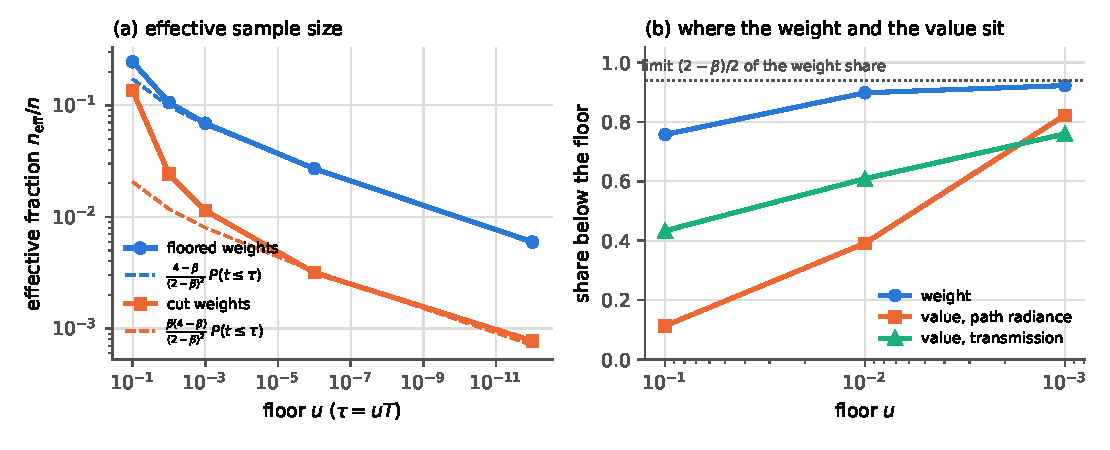
\includegraphics[width=\textwidth]{fig_weight}
\caption{(a) The effective fraction $n_{\rm eff}/n$ of the floored weights $\max\{t,\tau\}^{-2}$ and of the cut weights
$t^{-2}\1\{t>\tau\}$ over the entries of the physical domain of the EMIT table, $\tau=uT$ with $T$ the median
transmission, and the limits of Proposition~\ref{prop:neff} at $\beta=0.12$. (b) On the test block of one EMIT split,
the share of the floored weight on the entries below the floor, and the share of the floored objective's value there
at the residuals of the plain network, for the path radiance and the transmission; the dotted line is the limit of
Corollary~\ref{cor:below}.}\label{fig:weight}
\end{figure}

Mixing the two objectives buys effective sample size back once $\alpha$ is small against $\sqrt{\rho_\tau}$. With
$\bar w_\tau=w_\tau/\E_p[w_\tau]$ and $\rho_\tau=1/\E_p[\bar w_\tau^2]$, the weights $w=(1-\alpha)+\alpha\bar w_\tau$
have mean one and effective fraction $1/(1-\alpha^2+\alpha^2/\rho_\tau)$, while $\E_p[\bar w_\tau e_R^2]\le\E_p[w\,e_R^2]
/\alpha$ keeps the retrieval certificate up to the factor $1/\alpha$. For the path radiance in the coordinates of
training at $u=10^{-2}$, where $\rho_\tau=0.021$, the fraction is $0.89$, $0.35$ and $0.08$ at $\alpha=0.05$, $0.2$ and
$0.5$.

\begin{corollary}[rate against effective sample size]\label{cor:neff-rate}
Under the hypotheses of Proposition~\ref{prop:neff}, suppose a plain fit on $n$ entries has $\E_p[e_R^2]\le Cn^{-\gamma}$
and a fit with the normalized floored weights $\bar w_\tau$ has $\E_p[\bar w_\tau e_R^2]\le Cn_{\rm eff}^{-\gamma}$ with
$n_{\rm eff}=n\,\E_p[w_\tau]^2/\E_p[w_\tau^2]$, for some $\gamma>0$. With the floor chosen as a power of $n$,
\[
\E_p|\bar\rho-\rho|^2=O\bigl(n^{-\beta\gamma/(2+\beta)}\bigr)\ \text{(plain)},\qquad
\E_p|\bar\rho-\rho|^2=O\bigl(n^{-\beta\gamma/(2+\beta\gamma)}\bigr)\ \text{(floored weights)},
\]
so the weighted exponent is the larger exactly when $\gamma<1$.
\end{corollary}

\begin{proof}
For both fits $\E_p|\bar\rho-\rho|^2\le R^2F(\tau)+\E_p[t^{-2}e_R^2\1\{t>\tau\}]$. For the plain fit the second term is
at most $\tau^{-2}Cn^{-\gamma}$, and $\tau=n^{-\gamma/(2+\beta)}$ balances it against $R^2F(\tau)\sim R^2A\tau^\beta$.
For the weighted fit $t^{-2}\1\{t>\tau\}\le w_\tau$, so the second term is at most $\E_p[w_\tau]\,Cn_{\rm eff}^{-\gamma}$,
which by Proposition~\ref{prop:neff} is of order $\tau^{\beta-2}(n\tau^\beta)^{-\gamma}$; $\tau=n^{-\gamma/(2+\beta\gamma)}$
balances it.
\end{proof}

On EMIT the learning curves of \cite{shmalo2} give mean-square exponents of about $0.8$ to $1.2$ on the first three
components, and with $\beta\approx0.12$ the two exponents agree to within about one percent either way. Rates cannot
decide whether weighting pays on this table; the constants decide it, and Section~\ref{sec:networks} measures them.

\section{Choosing on the retrieval error}\label{sec:choosing}

Fitting a model on a weighted objective pays the effective sample size of the entries. Choosing among a few candidates
fitted on the forward error pays much less, because the choice is made on a sum over states.

\begin{proposition}[choosing on a weighted criterion]\label{prop:select}
Let $Z_1,\dots,Z_m$ be independent copies of a state $Z$ with $B$ entries, let $v_b(Z)\ge0$ be entry weights with state
weight $\omega(Z)=\sum_bv_b(Z)\le\omega_{\max}$, and let $\ell_{k,b}(Z)\in[0,L]$ be the entry losses of $K$ candidates.
Put $R_k=\E\sum_bv_b\ell_{k,b}$, let $\hat R_k$ be its mean over the $m$ states, and let
$m_{\rm eff}=m\,\E[\omega]^2/\E[\omega^2]$. With probability at least $1-\delta$ the candidate $\hat k$ that minimizes
$\hat R_k$ satisfies
\[
R_{\hat k}-\min_kR_k\le2L\,\E[\omega]\Bigl(\sqrt{\frac{2\log(2K/\delta)}{m_{\rm eff}}}
+\frac{2\omega_{\max}}{3\,\E[\omega]}\,\frac{\log(2K/\delta)}{m}\Bigr).
\]
\end{proposition}

\begin{proof}
The state loss $X_k=\sum_bv_b\ell_{k,b}$ lies in $[0,L\omega_{\max}]$ and has
$\operatorname{Var}X_k\le\E X_k^2\le L^2\E[\omega^2]=L^2\E[\omega]^2m/m_{\rm eff}$. With $x=\log(2K/\delta)$, Bernstein's
inequality gives $|\hat R_k-R_k|\le\varepsilon$ with $\varepsilon=\sqrt{2x\operatorname{Var}X_k/m}+2L\omega_{\max}x/(3m)$
except on an event of probability at most $\delta/K$, and a union bound over $k$ makes this hold for every $k$ with
probability at least $1-\delta$. Then $R_{\hat k}\le\hat R_{\hat k}+\varepsilon\le\hat R_{k^\ast}+\varepsilon\le
R_{k^\ast}+2\varepsilon$ for the best candidate $k^\ast$, and $2\varepsilon$ is at most the stated bound.
\end{proof}

The weights enter only through the effective number of states and the ratio $\omega_{\max}/\E[\omega]$. On an EMIT
validation block of $m=2{,}098$ states the cut weights keep $1{,}962$, $1{,}831$ and $1{,}639$ effective states at
$u=10^{-1},10^{-2},10^{-3}$, with $\omega_{\max}/\E[\omega]$ between $2.6$ and $3.0$, and the floored weights $1{,}917$,
$1{,}763$ and $1{,}579$. For $K=32$ and $\delta=0.05$ the bound is $0.18$ to $0.20$ times $L\,\E[\omega]$, against
$0.17$ with no weights at all: weighting the criterion raises the price of choosing by eight to eighteen percent, while
it divides the effective data of a weighted fit by fourteen at $u=10^{-3}$.

A convex stack is a choice of this kind with a continuum of candidates. For members with component errors $e^{(j)}$ and
weights $w$ on a product $W$ of simplices, write $F(w)$ and $G(w)$ for the first-order forward and retrieval errors of
the stack; both are convex quadratics in $w$.

\begin{proposition}[the mixtures trace the frontier]\label{prop:pareto}
Let $W$ be a product of simplices and $F(w)=w^\top Bw$, $G(w)=w^\top Aw$ with $A,B$ positive semidefinite. If $w^\ast\in
W$ is weakly Pareto optimal for $(F,G)$, that is, no $w\in W$ has $F(w)<F(w^\ast)$ and $G(w)<G(w^\ast)$, then $w^\ast$
minimizes $\alpha F+(1-\alpha)G$ over $W$ for some $\alpha\in[0,1]$.
\end{proposition}

\begin{proof}
The set $S=\{(F(w),G(w))+u:\ w\in W,\ u\in[0,\infty)^2\}$ is convex, since $F$ and $G$ are convex and $W$ is convex.
Weak optimality says that $(F(w^\ast),G(w^\ast))-(0,\infty)^2$ does not meet $S$, so the point lies on the boundary of $S$,
and a supporting line gives $\lambda\neq0$ with $\lambda\cdot s\ge\lambda\cdot(F(w^\ast),G(w^\ast))$ for all $s\in S$.
Since $S$ is closed upward, $\lambda\ge0$; normalize $\lambda$ to $(\alpha,1-\alpha)$.
\end{proof}

\begin{lemma}[the path is monotone]\label{lem:monotone}
For $0\le\alpha_1<\alpha_2\le1$ let $w_i$ minimize $\alpha_iF+(1-\alpha_i)G$ over $W$. Then $F(w_2)\le F(w_1)$ and
$G(w_2)\ge G(w_1)$.
\end{lemma}

\begin{proof}
Write $x=F(w_1)-F(w_2)$ and $y=G(w_2)-G(w_1)$. Optimality of $w_1$ and of $w_2$ gives $\alpha_1x\le(1-\alpha_1)y$ and
$(1-\alpha_2)y\le\alpha_2x$. Multiplying the first by $1-\alpha_2$ and the second by $1-\alpha_1$ and chaining,
$(1-\alpha_2)\alpha_1x\le(1-\alpha_1)\alpha_2x$, that is $(\alpha_2-\alpha_1)x\ge0$, so $x\ge0$. Then the first
inequality gives $(1-\alpha_1)y\ge\alpha_1x\ge0$, so $y\ge0$.
\end{proof}

The proof of Proposition~\ref{prop:pareto} uses only that $W$ is convex and that $F$ and $G$ are convex on it, so the
same holds for any convex class of predictors, for instance the functions of norm at most $r$ in a reproducing kernel
Hilbert space; kernel ridge regression with the entry weights $(1-\alpha)+\alpha g/\bar g$ is the penalized form of
that problem.

\section{Tables, emulators and scores}\label{sec:data}

\paragraph{EMIT.} The first table has $23{,}313$ evaluations of a radiative-transfer code provided by the Jet
Propulsion Laboratory as a lookup table for EMIT atmospheric correction. The input is the atmospheric and viewing
state in $\mathbb R^6$ (aerosol optical depth, surface elevation, water-vapour column, relative azimuth, solar and view
zenith angles), and the output is four spectral components on the $285$-point EMIT grid from $381$ to $2493$\,nm: path
radiance $Y_1=a$, direct and diffuse fluxes $Y_2$ and $Y_3$ with $t=Y_2+Y_3$, and spherical albedo $Y_4=s$
\cite{shmalo2}. Each split draws a test block of $2{,}331$ states and a validation block of $2{,}098$ from a seeded
permutation and fits on the remaining $18{,}884$; the splits are the ten seeds $101$--$110$ of \cite{shmalo2}. The two
failed evaluations of Section~\ref{sec:price}, states $4011$ and $7439$, are both in the training block on eight splits;
split $104$ has one in its test block and split $105$ one in its validation block. The networks of
Section~\ref{sec:networks} are fitted with them and, removed from whichever block holds them, without them; the members
of the stacks of Section~\ref{sec:stacks}, the kernels of Section~\ref{sec:kernels} and the networks of
Section~\ref{sec:epochs} are fitted on the table as provided.

\paragraph{libRadtran.} The second table is the libRadtran half of the corpus of \cite{pkan} over the thirteen
Sentinel-2 bands, restricted to the $9{,}722$ states that carry all thirteen: the path reflectance, total
transmittance and spherical albedo for each state and band, with the seven continuous state variables and the one-hot
aerosol model and atmosphere profile as inputs \cite{shmalo2}. Twelve of the thirteen bands keep a transmission above
$0.14$ on every state; band B10 at $1372$\,nm, in a strong water-vapour band, holds every smaller transmission. The
splits use the same seeds and proportions ($972$ test, $7{,}875$ fitting states).

\paragraph{The published libRadtran benchmark.} The release of \cite{pkan} pairs 6S and libRadtran values of the path
reflectance $a$, the total transmittance $t$ and the spherical albedo $s$ for $50{,}000$ states over the thirteen
Sentinel-2 bands of \cite{drusch2012}, with its own state-level split into $35{,}000$ training, $7{,}500$ validation and
$7{,}500$ test states and its own code for the metrics. Its files hold $609{,}722$ of the $650{,}000$ rows of one state
and one band, the rest removed by its quality control, and we fit and score on the rows present, $426{,}761$, $91{,}490$
and $91{,}471$. Each row is fitted separately and the band enters through the
inputs: eight state and band variables and the one-hot aerosol model and atmosphere profile, to which we add the 6S
coefficients of the same row, and the network predicts the libRadtran coefficients minus the 6S ones, the residual form
of the release's best models. The networks have four hidden layers of $384$ SiLU units \cite{silu} and three outputs,
are trained with Adam \cite{adam} and a one-cycle schedule \cite{onecycle} for $80$ epochs at batch size $1{,}024$, and
are kept at the epoch with the lowest validation value of their own objective. The weighted arms use the weights of
$J_u$ row by row at the true transmission, $\max\{t,\tau\}^{-2}$, $R^2\max\{t,\tau\}^{-2}$ and $R^4t^2\max\{t,\tau\}^{-2}$
for the three coefficients with $\tau=uT_{\rm train}$, each normalized to mean one on the training rows. The forward
scores are the release's: the root-mean-square, mean absolute and symmetric mean absolute percentage errors over the
three coefficients of every test row, and $R^2$ averaged over the coefficients. The retrieval scores are those below,
with the top-of-atmosphere reflectance $a+\rho t/(1-\rho s)$ in the role of the radiance.

\paragraph{Emulators.} The members are the six families of \cite{shmalo2}: a cubic ridge regression, Mat\'ern kernel
ridge regression on the inputs with an isotropic and with an input-scaled metric, a network of three hidden layers of
$512$ units, the network with a kernel correction of its residuals, and kernel ridge regression on the network's last
hidden features. The kernel regressions are fitted on the full fitting block in the space of the leading $64$
principal components of each standardized component, with their hyperparameters chosen on the validation block; the
network is trained with AdamW and a cosine schedule for up to $150$ epochs and stopped on the validation loss with a
patience of $25$ epochs. The convex stacks of \cite{wolpert,breiman} combine the six members with weights on a simplex
for each component.

\paragraph{Scores.} All scores are on the test block, at $\rho=0.7$: the mean relative $\ell^2$ error of the radiance
across bands, and the 95th percentile of the retrieval error $|\hat\rho-\rho|$, in points of reflectance ($100$ times
the absolute error), over all entries and over the physical domain above $fT_{\rm train}$ for $f=10^{-12},10^{-3},
10^{-2}$, that is, the entries with $t\ge fT_{\rm train}$, $0\le s<1$ and $1-\rho s\ge0.3$, where a failed inversion is
counted as a failure and left out of the percentile \cite{shmalo2}.

\section{Experiments}\label{sec:experiments}

\subsection{Networks fitted on the retrieval error}\label{sec:networks}

The network of Section~\ref{sec:data} is trained on each component with the weights of the first-order bound,
\[
J_u=\E\Bigl[\frac{e_a^2+R^2(e_{Y_2}^2+e_{Y_3}^2)+R^4t^2e_s^2}{\max\{t,uT_{\rm train}\}^2}\Bigr],\qquad R=0.9,
\]
normalized to mean one on the training block of each component and stopped on the same weighted loss of the
validation block (the \emph{floored} arms). Three variants change one thing each: the floored weights at $u=10^{-2}$
stopped on the plain validation loss, the mixed weights $(1-\alpha)+\alpha\bar w_\tau$ of Section~\ref{sec:price} with
$\alpha=0.2$ at $u=10^{-2}$, and the cut weights $v_\tau$ of Proposition~\ref{prop:neff} at $u=10^{-2}$, normalized and
used for stopping in the same way. The \emph{flattened} arms raise the floored weights to a power $\kappa\in(0,1)$, the
device Shimodaira proposed for covariate shift \cite{shimodaira}, and normalize them to mean one in the same way: at
$u=10^{-2}$ with $\kappa=1/4$ and $\kappa=1/2$, and with $\kappa=1/4$ stopped on the plain validation loss at $u=10^{-2}$
and $10^{-3}$. For the path radiance and the two fluxes the flattened weights at $\kappa$ are, above the floor, those of
the certificate of Proposition~\ref{prop:weighted-rate} at $\alpha=\kappa$; the albedo's become constant above the
floor. We write $K_u$ for the objective $J_u$ with $v_\tau$ in place of the floored weights.
The \emph{joint} arms train one network for all four components on the first-order retrieval error at
$\rho\in\{0.1,0.4,0.7\}$ with $t$ floored at $uT_{\rm train}$, plus $10^{-2}$ times the standardized squared error.
Every run also fits the plain network on the same split with the same seed. Training is deterministic: on the table as
provided the plain networks of the different runs agree to four decimals of the radiance error on every split, so
every difference below is paired. Run on the table as provided, the code behind the upper block of
Table~\ref{tab:networks} reproduces the runs of its lower block on splits $101$ and $105$, every arm to four decimals of
every score on the same machine, so the two blocks differ in the two failed evaluations alone. Table~\ref{tab:networks} gives the differences on the EMIT table without its two
failed evaluations and, in its lower block, on the table as provided. Without the failed evaluations the plain network
has a radiance error of $0.350\%$, an all-band tail of $64.9$ points and physical tails of $9.7$, $3.5$ and $2.1$ points
at the three floors.

\begin{table}[t]
\centering\footnotesize\setlength{\tabcolsep}{3pt}
\resizebox{\textwidth}{!}{%
\begin{tabular}{@{}lcccccc@{}}
\toprule
arm & radiance [pp] & all bands & phys.\ $10^{-12}$ & phys.\ $10^{-3}$ & phys.\ $10^{-2}$ & failed [pp]\\
\midrule
% network-table-rows: begin
\multicolumn{7}{@{}l}{\emph{without the two failed evaluations}}\\
floored, $u=10^{-1}$ & $-0.01\pm0.01$ (9) & $-8.7\pm2.4$ (10) & $-2.3\pm1.3$ (10) & $-1.3\pm0.2$ (10) & $-0.7\pm0.1$ (10) & $-0.07$\\
floored, $u=10^{-2}$ & $+0.26\pm0.02$ (0) & $-19.9\pm2.6$ (10) & $-2.2\pm1.2$ (10) & $-0.1\pm0.2$ (7) & $+0.6\pm0.1$ (0) & $-0.10$\\
floored, $u=10^{-3}$ & $+1.33\pm0.05$ (0) & $+3.1\pm1.9$ (0) & $+26.9\pm2.3$ (0) & $+15.2\pm1.0$ (0) & $+13.1\pm0.7$ (0) & $-0.10$\\
floored, $u=10^{-2}$, plain stopping & $+0.26\pm0.01$ (0) & $-19.9\pm2.6$ (10) & $-2.2\pm1.3$ (10) & $-0.1\pm0.2$ (6) & $+0.6\pm0.1$ (0) & $-0.10$\\
mixed, $\alpha=0.2$, $u=10^{-2}$ & $-0.00\pm0.01$ (5) & $-6.5\pm2.0$ (10) & $-1.4\pm1.1$ (9) & $-0.4\pm0.2$ (10) & $-0.1\pm0.1$ (8) & $-0.08$\\
flattened, $\kappa=0.25$, $u=10^{-2}$ & $-0.03\pm0.01$ (10) & $-12.3\pm2.6$ (10) & $-3.0\pm1.4$ (10) & $-1.0\pm0.2$ (10) & $-0.5\pm0.1$ (10) & $-0.08$\\
flattened, $\kappa=0.5$, $u=10^{-2}$ & $-0.03\pm0.01$ (10) & $-24.8\pm3.0$ (10) & $-4.3\pm1.3$ (10) & $-1.5\pm0.2$ (10) & $-0.7\pm0.1$ (10) & $-0.10$\\
flattened, $\kappa=0.25$, $u=10^{-2}$, plain stopping & $-0.02\pm0.01$ (10) & $-12.4\pm3.0$ (10) & $-2.6\pm1.7$ (9) & $-1.0\pm0.2$ (10) & $-0.5\pm0.1$ (10) & $-0.08$\\
flattened, $\kappa=0.25$, $u=10^{-3}$, plain stopping & $-0.02\pm0.01$ (10) & $-23.4\pm3.5$ (10) & $-3.0\pm1.3$ (10) & $-1.0\pm0.2$ (10) & $-0.4\pm0.1$ (10) & $-0.09$\\
cut, $u=10^{-2}$ & $+0.32\pm0.02$ (0) & $+5.6\pm1.8$ (0) & $-6.5\pm1.4$ (10) & $-0.8\pm0.2$ (10) & $-0.0\pm0.1$ (6) & $+0.98$\\
joint, $u=10^{-2}$ & $+0.17\pm0.02$ (0) & $-27.1\pm1.8$ (10) & $-2.4\pm1.4$ (9) & $-0.1\pm0.2$ (6) & $+0.5\pm0.1$ (0) & $-0.10$\\
joint, $u=10^{-3}$ & $+0.83\pm0.03$ (0) & $-8.1\pm2.9$ (10) & $+23.6\pm2.0$ (0) & $+13.7\pm1.2$ (0) & $+11.8\pm0.9$ (0) & $-0.10$\\
\midrule
\multicolumn{7}{@{}l}{\emph{the table as provided}}\\
floored, $u=10^{-1}$ & $+0.55\pm0.16$ (0) & $+0.9\pm2.6$ (4) & $+2.2\pm1.6$ (2) & $+1.5\pm0.5$ (0) & $+1.3\pm0.4$ (0) & $+0.05$\\
floored, $u=10^{-2}$ & $+5.56\pm5.08$ (0) & $+18.6\pm45.5$ (1) & $+45.5\pm53.7$ (0) & $+38.9\pm59.5$ (0) & $+37.9\pm60.6$ (0) & $+0.02$\\
floored, $u=10^{-3}$ & $+18.55\pm1.77$ (0) & $+350.8\pm142.8$ (0) & $+397.8\pm137.0$ (0) & $+413.1\pm140.8$ (0) & $+403.6\pm144.8$ (0) & $+0.15$\\
joint, $u=10^{-2}$ & $+0.85\pm0.24$ (0) & $-20.1\pm5.3$ (10) & $+2.7\pm4.5$ (3) & $+2.5\pm1.0$ (0) & $+2.7\pm0.8$ (0) & $-0.09$\\
joint, $u=10^{-3}$ & $+6.26\pm3.25$ (0) & $+28.0\pm56.1$ (0) & $+70.6\pm55.9$ (0) & $+67.4\pm59.8$ (0) & $+63.5\pm54.6$ (0) & $-0.04$\\
% network-table-rows: end
\bottomrule
\end{tabular}}
\caption{Networks fitted on the retrieval error, EMIT: difference from the plain network of the same run in the radiance
error and in the 95th percentiles of the retrieval error (points), mean $\pm$ standard deviation over splits, with the
number of splits on which the arm is lower in parentheses, and the mean difference in the share of failed inversions
on the physical domain above $10^{-3}T_{\rm train}$. Floored: weights $\bar w_\tau$; mixed: $(1-\alpha)+\alpha\bar w_\tau$;
flattened: $\bar w_\tau^{\,\kappa}$ renormalized; cut: $v_\tau$; joint: one network for all four components. Upper block:
the table without its two failed evaluations, splits $101$--$110$; lower block: the table as provided, splits
$101$--$110$.}\label{tab:networks}
\end{table}

Without the failed evaluations the floored weights at $u=10^{-1}$ improve on the plain network in every tail on every
split. The tails on the physical domain fall by nearly a quarter at $10^{-12}T_{\rm train}$ and by more than a third at
$10^{-3}$ and $10^{-2}$, the all-band tail falls by $8.7$ points, the share of failed inversions above
$10^{-3}T_{\rm train}$ falls from $0.10\%$ to $0.04\%$, and the radiance error falls by $0.01$ percentage points, on
nine splits of ten. On the test blocks the network has the lower value of the floored objective at all three floors
on every split, by median factors of $0.64$, $0.42$ and $0.56$ at $u=10^{-1},10^{-2},10^{-3}$, and of $K_u$ at
$10^{-2}$ and $10^{-3}$ on every split ($0.36$ and $0.42$). The components move apart: the network lowers the error of
the path radiance by a quarter and that of the direct flux by nearly a tenth, and it triples that of the albedo, from $1.6\%$
to $4.8\%$. The albedo weights of $J_u$, $R^4t^2/\max\{t,\tau\}^2$, vanish with the transmission, and so does the fit:
on split $101$ the network's albedo error is $0.64\%$ against $0.70\%$ on the entries above $10^{-1}T_{\rm train}$,
and $11.5\%$ against $3.8\%$ on those between $10^{-2}$ and $10^{-1}T_{\rm train}$.

At the lower floors the objective and the tails part. The floored network at $u=10^{-2}$ has the lower value of its
objective on held-out states on every split (median factor $0.84$) and trades one error for another: its all-band tail
falls by $20$ points and its tail above $10^{-12}T_{\rm train}$ by $2.2$, while its radiance error rises by $0.26$
percentage points and its tail above $10^{-2}T_{\rm train}$ by $0.55$. At $u=10^{-3}$ the objective is again lower on
every split ($0.54$), and every error rises, the radiance error by $1.3$ points and the physical tails by $13$ to $27$.
The joint arms, one network for all four components, trade the same way and a little more cheaply: at $u=10^{-2}$ the
all-band tail falls by $27$ points on every split for a rise of $0.17$ percentage points in the radiance error, and at
$10^{-3}$ the physical tails rise by $12$ to $24$ points.
The objective is a mean, and at $u=10^{-3}$ most of its value sits on the entries below the floor
(Section~\ref{sec:price}); a network can lower it there while the 95th percentile, which the rest of the physical
domain sets, grows. Nor are the lower floors attained best by the networks fitted on them. On held-out states the
lowest $J_{10^{-2}}$ belongs to the network fitted at $u=10^{-1}$ on nine splits of ten and to the mixed weights on
the tenth, never to the network fitted on it (median factor $0.42$ against $0.84$), and the lowest $J_{10^{-3}}$ to a
network fitted at $u=10^{-2}$ on every split ($0.15$ against $0.54$). The cut weights make the point most plainly: the
network fitted on $K_{10^{-2}}$ has a higher value of it on held-out states than the plain network on nine splits of
ten (median factor $1.21$), against $0.36$ for the floored network at $u=10^{-1}$. In the coordinates of training the
floored weights at $u=10^{-1}$ keep an effective fraction of $0.046$ to $0.072$ of the entries of the first three
components, against $0.016$ to $0.024$ at $u=10^{-2}$ and $0.007$ to $0.013$ for the cut weights there, and at the
size of this table the entries a higher floor keeps are worth more than a closer match between the objective fitted and
the objective scored.

Stopping on the plain validation loss moves none of the mean differences at $u=10^{-2}$ by more than $0.07$ points
(on a single split by at most $1.4$ points, in the all-band tail), so the trade comes from the training weights and not
from the stopping rule. The mixture with $\alpha=0.2$ lowers the
tails on average at an unchanged radiance error, by less than the floored weights at $u=10^{-1}$ on each of the five
errors of the table. The cut weights
appear to lower the tail above $10^{-12}T_{\rm train}$ by $6.5$ points, but a failed inversion is left out of the
percentile. The cut network fails on $1.1\%$ of the entries above $10^{-3}T_{\rm train}$, against $0.1\%$ for the
plain network, and on more than $5\%$ of those above $10^{-12}T_{\rm train}$ on every split, so that its tail there is
infinite once the failures are counted. Counting every failure as an infinite error, on split $101$ the tail above
$10^{-3}T_{\rm train}$ is $3.26$ points for the cut network, $3.23$ for the plain one and $2.19$ for the floored
network at $u=10^{-1}$, and $3.8\%$, $3.5\%$ and $2.6\%$ of the entries have an error above five points.

Flattening the weights does better than any floor. At $u=10^{-2}$ and $\kappa=1/2$, weights proportional to
$1/\max\{t,\tau\}$ for the path radiance and the fluxes, the network lowers the radiance error on every split, from
$0.350\%$ to $0.322\%$ on average ($8\%$, split by split $5$ to $10\%$), and every tail on every split: the all-band
tail from $64.9$ to $40.1$ points and the physical tails from $9.7$, $3.5$ and $2.1$ to $5.3$, $2.0$ and $1.4$ points,
by $44$, $42$ and $32\%$ on average (split by split $28$--$57\%$, $35$--$44\%$ and $26$--$37\%$). The share of failed
inversions above $10^{-3}T_{\rm train}$ falls from $0.10\%$ to $0.005\%$. Against the floored network at $u=10^{-1}$
it is lower in the radiance error, the all-band tail and the tails above $10^{-12}$ and $10^{-3}T_{\rm train}$ on every
split, and higher in the tail above $10^{-2}T_{\rm train}$ on nine splits of ten ($1.38$ against $1.32$ points on
average). It lowers the errors of the path radiance, the direct flux and the diffuse flux on every split (medians
$0.49\%$ to $0.37\%$, $0.95\%$ to $0.86\%$ and $0.39\%$ to $0.38\%$) and raises the albedo's on every split, from
$1.56\%$ to $2.24\%$, against a tripling at $u=10^{-1}$. It also attains the weighted objectives on held-out states
better than the networks fitted on them: of all the networks fitted on one component at a time it has the lowest value
of $J_{10^{-2}}$, $K_{10^{-2}}$ and $K_{10^{-3}}$ on every split, of $J_{10^{-1}}$ on nine and of $J_{10^{-3}}$ on six, with
median factors against the plain network of $0.19$ for $J_{10^{-2}}$, where the network fitted on $J_{10^{-2}}$ reaches
$0.84$, and of $0.54$ for $J_{10^{-1}}$, where the network fitted on it reaches $0.64$. The weights with $\kappa=1/4$
give the same radiance error and most of the gain in the tails ($30$, $30$ and $25\%$ on the physical domain), and
stopping them on the plain validation loss moves each of these averages by at most five points. None of this is explained by the effective
sample size alone. Over the entries of the table the flattened weights at $u=10^{-2}$ keep an effective fraction of
$0.37$ at $\kappa=1/4$ and $0.15$ at $\kappa=1/2$, against $0.11$ for the floored weights at that floor and $0.24$ at
$u=10^{-1}$: the best network keeps fewer effective entries than the floored network at $u=10^{-1}$. What flattening
keeps, and a higher floor gives up, is the order of the weights between $10^{-2}$ and $10^{-1}T_{\rm train}$, where a
floor at $10^{-1}$ makes them equal; what it removes is most of their range, a factor of $100$ between $10^{-2}$ and
$1$ times $T_{\rm train}$ instead of $10^4$.

The floor itself can be chosen on the validation block. A second set of runs trains the network on the floored
weights at six floors, $u\in\{10^{3},1,0.3,0.1,0.03,0.01\}$, on each split, and keeps the one with the lowest cut
objective $K_{10^{-2}}$ on the validation block, a rule fixed before the runs. On the EMIT table it picks $u=10^{-1}$ on
every split, the floor whose network also has the lowest tail above $10^{-3}T_{\rm train}$ on the test block, and so it
reproduces the first row of Table~\ref{tab:networks}: the four tails fall by $8.7$, $2.3$, $1.3$ and $0.73$ points on
every split at an unchanged radiance error. The floors on either side trade in opposite directions. At $u=1$ and above
the floored weights are nearly constant in the transmission and the fit is a least-squares fit in physical units: it
lowers the radiance error by $0.10$ percentage points on every split, from $0.35\%$ to $0.25\%$, and raises the tails
on average, the one above $10^{-12}T_{\rm train}$ by $4$ to $10$ points. Weighting by the band variance alone does the
same to within $0.05$ points in every score, so the albedo weights play no part there. At $u=0.03$ the all-band tail
falls by $19$ points and the radiance error rises by $0.08$, the trade of $u=10^{-2}$ on a smaller scale. The rule
settles on the one floor that improves both.

With the failed evaluations (lower block) every floored and joint arm raises the radiance error and the tails above
$10^{-3}$ and $10^{-2}T_{\rm train}$ on every split, and only the joint arm at $u=10^{-2}$ has a lower all-band tail on
all ten. With the failed states the plain network has the lower value of the weighted objective itself on the test blocks
of nine, nine and ten of the ten splits at $u=10^{-1},10^{-2},10^{-3}$, by median factors of $4.3$, $9.9$ and $8.3$,
while on the training blocks of splits $101$--$103$ the weighted network reaches $0.03$ to $0.06$ of the plain network's
value: it fits the entries that carry its objective and does not generalize from them. Two effects of the failed states combine. At
$u=10^{-2}$ and $10^{-3}$ they leave the floored weights of the path radiance $75$ and $10$ effective training states
(Section~\ref{sec:price}). At $u=10^{-1}$ they hold under one percent of the weight, but no smooth fit returns a zero
flux between neighbours with ordinary ones, and their share of the value of the objective is far larger. On split
$104$, whose test block holds one of them, the ratio of the floored objective of the plain network's residuals to their
plain mean square is $23$ for the direct flux and $86$ for the diffuse flux at $u=10^{-1}$, against $0.12$ to $0.42$ and
$0.24$ to $0.55$ on the other nine splits: that one state carries about $99\%$ of the objective of each flux. The
weighted network at $u=10^{-1}$ loses its accuracy on those two components, with errors of $2.4\%$ and $0.90\%$ on split
$101$ against $0.86\%$ and $0.40\%$ without the failed states. The split that puts a failed state in the validation block,
$105$, is the worst of all, since the weighted stopping rule there is decided by that state; at $u=10^{-2}$ its tail
above $10^{-2}T_{\rm train}$ rises by $208$ points, against $7$ to $44$ on the other splits. The failed states also cost
the plain network part of its accuracy. Removing them lowers its radiance error on each of the ten splits, by $0.035$
percentage points on average, and its albedo error from $2.93\%$ to $1.57\%$, while its physical tails move by less
than a quarter of a point, up on some splits and down on others.

On the libRadtran table, which has no failed evaluations, the floored and joint arms raise the radiance error on every
split, by $0.03$ to $0.48$ percentage points against a plain error of $0.356\%$, and the tail above $10^{-3}T_{\rm
train}$ on nine or ten splits of ten. There the floored weights put $86\%$, $99.8\%$ and essentially all of their mass
on band B10 at the three floors, so that the network is asked to fit one band of thirteen, the band where the
retrieval is ill-conditioned, at the expense of the other twelve. The rule that chooses the floor on the validation
block fails there. It picks $u=10^{-2}$ on every split, the floor closest to its own criterion, and that network raises
the radiance error by $0.06$ percentage points and the tails above $10^{-3}$ and $10^{-2}T_{\rm train}$ by $0.12$
points on every split, and lowers only the all-band tail, by $2.6$ points on nine splits. No floor improves on the
plain network there in both the radiance error and the tails: at $u=1$ and above the radiance error falls by $0.02$ percentage points or less on
average and the tail above $10^{-3}T_{\rm train}$ moves by less than $0.11$ points on every split, while the all-band
tail rises by $34$ points.

\subsection{The published libRadtran benchmark}\label{sec:pkan}

On the benchmark of \cite{pkan} (Section~\ref{sec:data}) the plain network stands near the release's models in their
own metrics (Table~\ref{tab:pkan}). Its RMSE over five seeds, $0.00669$, lies between that of pKANrtm, $0.00619$, and
that of sRTMnet \cite{brodrick} as trained in the release, $0.00691$, and below those of the release's five other
baselines, $0.00784$ to $0.01394$; a residual network tuned for this split in \cite{shmalo2} reaches $0.00581$.

The two weighted networks trade one of the release's metrics against the others, on each of the five seeds. The
floored weights at $u=10^{-1}$ and the flattened weights with $\kappa=1/2$ at $u=10^{-2}$ lower the mean absolute error
to $0.00083$ and $0.00069$, $0.45$ and $0.37$ of pKANrtm's and below every model of the release, and the symmetric
percentage error to $2.13\%$ and $1.96\%$, against $3.91\%$ for pKANrtm and $4.13\%$ for the plain network. They raise
the RMSE to $0.00785$ and $0.00792$, $1.27$ and $1.28$ times pKANrtm's and about that of the release's third model, and
lower $R^2$, which averages over the three coefficients, to $0.990$, above only the release's weakest baseline. The RMSE
pools the three coefficients, and the spherical albedo sets it: the albedo's error rises from $0.0094$ to $0.0134$ and
$0.0136$, while the errors of the path reflectance and of the transmittance fall by factors of $2.4$ and $2.7$ and of
$3.1$ and $3.9$. The albedo's retrieval weight vanishes with the transmission, as on the EMIT table
(Section~\ref{sec:networks}), and a single network with three outputs gives the capacity the other two weights ask for.

\begin{table}[t]
\centering\footnotesize\setlength{\tabcolsep}{3pt}
\resizebox{\textwidth}{!}{% generated by code/make_pkan_table.py from results/pkan; do not edit by hand
\begin{tabular}{@{}lcccccccc@{}}
\toprule
 & RMSE & MAE & $R^2$ & SMAPE [\%] & \multicolumn{3}{c}{RMSE by coefficient} & \\
\cmidrule(lr){6-8}
emulator & & & & & $\rho_{\rm path}$ & $T$ & $S$ & \\
\midrule
pKANrtm \cite{pkan} & $0.00619$ & $0.00186$ & $0.9947$ & $3.91$ & & & & \\
sRTMnet \cite{brodrick}, trained in \cite{pkan} & $0.00691$ & $0.00211$ & $0.9942$ & $4.28$ & & & & \\
DA \cite{pkan} & $0.00784$ & $0.00261$ & $0.9935$ & $4.95$ & & & & \\
GPAC \cite{pkan} & $0.00865$ & $0.00301$ & $0.9928$ & $5.58$ & & & & \\
FC \cite{pkan} & $0.00948$ & $0.00342$ & $0.9919$ & $6.13$ & & & & \\
RF \cite{pkan} & $0.01075$ & $0.00404$ & $0.9906$ & $7.02$ & & & & \\
UMR \cite{pkan} & $0.01394$ & $0.00546$ & $0.9869$ & $9.85$ & & & & \\
\midrule
6S as the emulator & $0.09790$ & $0.05348$ & $0.6386$ & $32.38$ & $0.02065$ & $0.16183$ & $0.04623$ & \\
network, plain & $0.00669\pm0.00043$ & $0.00225\pm0.00029$ & $0.9946\pm0.0005$ & $4.13\pm0.30$ & $0.00099\pm0.00009$ & $0.00666\pm0.00077$ & $0.00943\pm0.00042$ & \\
network, floored, $u=10^{-1}$ & $0.00785\pm0.00005$ & $0.00083\pm0.00002$ & $0.9899\pm0.0002$ & $2.13\pm0.02$ & $0.00041\pm0.00001$ & $0.00216\pm0.00007$ & $0.01341\pm0.00010$ & \\
network, flattened, $\kappa=1/2$, $u=10^{-2}$ & $0.00792\pm0.00002$ & $0.00069\pm0.00001$ & $0.9896\pm0.0001$ & $1.96\pm0.03$ & $0.00037\pm0.00001$ & $0.00170\pm0.00004$ & $0.01361\pm0.00004$ & \\
\midrule
 & radiance [\%] & all bands & phys.\ $10^{-12}$ & phys.\ $10^{-3}$ & phys.\ $10^{-2}$ & failed [\%] & & \\
\midrule
6S as the emulator & $20.565$ & $75.55$ & $75.55$ & $74.04$ & $73.81$ & $0.000$ & & \\
network, plain & $0.809\pm0.104$ & $3.21\pm0.21$ & $2.67\pm0.24$ & $2.38\pm0.20$ & $2.31\pm0.19$ & $0.097\pm0.025$ & & \\
network, floored, $u=10^{-1}$ & $0.225\pm0.008$ & $0.52\pm0.02$ & $0.48\pm0.02$ & $0.45\pm0.02$ & $0.44\pm0.01$ & $0.000\pm0.001$ & & \\
network, flattened, $\kappa=1/2$, $u=10^{-2}$ & $0.170\pm0.004$ & $0.48\pm0.01$ & $0.44\pm0.01$ & $0.41\pm0.01$ & $0.40\pm0.01$ & $0.000\pm0.000$ & & \\
\bottomrule
\end{tabular}
}
\caption{The published libRadtran benchmark of \cite{pkan}: test scores on the release's split. Upper block, the
release's metrics over the three coefficients of every test row, and the RMSE of each coefficient; the first seven rows
are the values published in Table~3 of the release for its model and its six baselines. Lower block, the
retrieval scores at $\rho=0.7$: the mean relative error of the top-of-atmosphere reflectance over the bands of a state,
the 95th percentiles of $|\hat\rho-\rho|$ in points over all rows and on the physical domain above $fT_{\rm train}$, and
the share of failed inversions above $10^{-3}T_{\rm train}$. Mean $\pm$ standard deviation over five seeds; 6S as the
emulator is the release's low-fidelity code scored as it stands.}\label{tab:pkan}
\end{table}

In the retrieval the weighted networks are better by a wide margin, again on every seed. The flattened network lowers
the radiance error from $0.81\%$ to $0.17\%$, the all-band 95th percentile from $3.21$ to $0.48$ points, the tails on the
physical domain from $2.67$, $2.38$ and $2.31$ to $0.44$, $0.41$ and $0.40$ points, and the share of failed inversions
above $10^{-3}T_{\rm train}$ from $0.097\%$ to $0.0002\%$; the floored network at $u=10^{-1}$ does nearly as well. 6S
scored as the emulator has a radiance error of $20.6\%$ and a tail of $75$ points, so the networks learn a correction of
it about two orders of magnitude smaller.

The result differs from that on the libRadtran table of Section~\ref{sec:data}, where no floor improved on the plain
network in both the radiance error and the tails. The two settings differ in three ways at once: the benchmark trains
on four and a half times as many states, its networks see the 6S coefficients and fit their residual, and they see one
band of a state at a time, with the band among the inputs, where the networks of the table predict all bands of a state
at once. The weighted networks were also still improving when training stopped: their lowest validation objective came
at epochs $78$ and $79$ of $80$ on every seed, against epochs $16$ to $28$ for the plain network.

\pending{a second set of runs on this benchmark, ten seeds at $300$ epochs with five hidden layers of $512$ units, adds
the flattened weights with the albedo left unweighted, a mixture with the plain objective, a kernel correction of each
network's residuals fitted on the same weights, an out-of-distribution split that tests on the states above the $0.85$
quantile of the aerosol optical depth or of the water-vapour column, as in \cite{shmalo2} (the release reports an RMSE
of $0.01022$ for pKANrtm on its own split of this kind), and ablations in $\kappa$ and $u$. Its results will replace the
last paragraph.}

\subsection{Kernel regression fitted on the retrieval error}\label{sec:kernelfit}

For kernel ridge regression the estimator of Section~\ref{sec:training} is the truncated reweighting of \cite{mpw}: for
each component and band,
\[
\min_f\ \sum_i w_i\bigl(f(x_i)-y_i\bigr)^2+\lambda\|f\|^2,\qquad \alpha_b=(K+\lambda W_b^{-1})^{-1}y_b ,
\]
with the entry weights of $J_u$ (floored) or $K_u$ (cut) at the true transmission. The weights change from band to band,
so every band is its own solve, and to keep $285$ solves per component affordable every arm is fitted on the same
$6{,}000$ training rows, the subsample on which the kernel's parameters are chosen, with the isotropic Mat\'ern kernel
and the smoothness, length scale and nugget the forward criterion chooses on the validation block. The weights are
scaled to mean one in each band, so that the nugget means the same in every arm, and the plain arm is the same solve
with $w=1$; the two forms of the normal equations, $(K+\lambda W_b^{-1})\alpha_b=y_b$ and
$(W_bK+\lambda I)\alpha_b=W_by_b$, give the same objectives to $10^{-13}$ on $300$ rows. On the table without its two
failed evaluations, over ten splits, the plain fit has a radiance error of $0.28\%$ and tails of $24.8$, $8.6$ and $5.0$
points on the physical domain (medians), against $0.075\%$ and $1.39$ points above $10^{-3}T_{\rm train}$ for the
input-scaled kernel of Section~\ref{sec:kernels}, which has its own length scales and is fitted on every training row.

The floored weights at $u=10^{-1}$ lower every physical tail on every split, by $15$, $13$ and $9\%$ at the median of
the paired ratios, lower their own objective on held-out states on every split (median factor $0.75$) and the share of
failed inversions above $10^{-3}T_{\rm train}$ from $0.67\%$ to $0.42\%$, and raise the radiance error on every split,
by $12\%$. At $u=10^{-2}$ the radiance error rises by $27\%$ and the tail above $10^{-12}T_{\rm train}$ falls by $28\%$,
while the one above $10^{-2}T_{\rm train}$ rises by $4\%$, each on every split, and the objective falls to $0.28$ of the
plain fit's. At $u=10^{-3}$ the objective falls to $0.08$ of the plain fit's, and the radiance error rises by $44\%$ and
the tails above $10^{-3}$ and $10^{-2}T_{\rm train}$ by $28$ and $53\%$, again on every split. The cut weights at
$10^{-2}$ lower the tails above $10^{-12}$ and $10^{-3}T_{\rm train}$ by $61$ and $23\%$ and multiply the radiance error
by $14$. The kernel repeats what the networks of Section~\ref{sec:networks} show: its objective on held-out states falls at
every floor, and the tails follow it only at the floor that keeps the most effective entries.

\subsection{Stacks chosen on the retrieval error}\label{sec:stacks}

The test states of each run are split in two halves; the weights of a stack are fitted on one half and scored on the
other, both ways, so that no state enters both the fit and its evaluation and no member saw a test state. The
\emph{component stack} has one simplex per component fitted on the mean relative error of that component, the
objective of the stack of \cite{shmalo2}; the \emph{retrieval stack} fits the four simplices jointly on the first-order
retrieval error $\sum(v_\rho^\top e)^2$ at $\rho=0.7$ over the entries of the physical domain with
$t\ge10^{-3}T_{\rm train}$.

On the EMIT table, over twenty runs (ten splits at network widths $512$ and $2000$) and $40$ held-out halves, the
component stack reproduces the reversal: its radiance error is lower than that of the kernel on features on all $40$
halves and its tail on the physical domain above $10^{-3}T_{\rm train}$ larger on all $40$. The retrieval stack has a
tail below the component stack's on $39$ of the $40$ halves and a higher radiance error on all $40$. Along the family
of Proposition~\ref{prop:pareto} the tail stays nearly flat while the radiance error falls until the weight on the
forward error is close to one (Figure~\ref{fig:frontier}).

\begin{figure}[t]
\centering
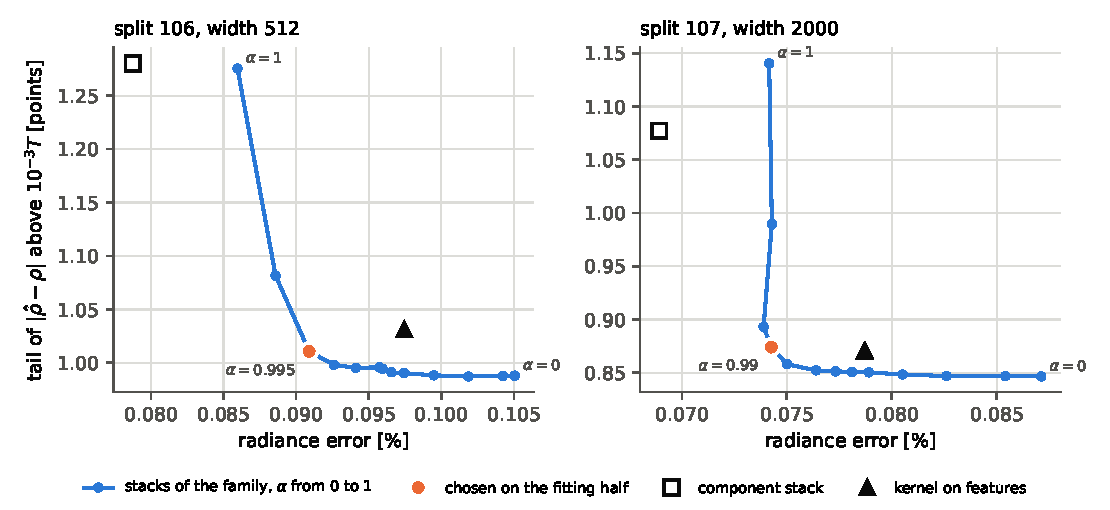
\includegraphics[width=\textwidth]{fig_frontier}
\caption{Stacks of the family of Proposition~\ref{prop:pareto} on one held-out half of two EMIT runs, from the
first-order retrieval error ($\alpha=0$) to the forward error at $\rho=0.7$ ($\alpha=1$): the radiance error against the
95th percentile of the retrieval error on the physical domain above $10^{-3}T_{\rm train}$. The orange point is the
stack whose $\alpha$ is chosen on the other half; the square is the component stack and the triangle the kernel on
learned features.}\label{fig:frontier}
\end{figure} With the mixture chosen on the fitting half alone, as the lowest radiance error among
the objectives whose tail on that half is no larger than that of the best single member, the chosen weight on the
forward error is at least $0.9$ on $36$ of the $40$ halves (median $0.99$), and the stack has a lower radiance error than
the kernel on features on $33$ of the $40$ held-out halves and a lower tail than the component stack on $39$, by $25\%$ at
the median (quartiles $20\%$ and $29\%$, at most $39\%$). Its tail lies between $0.06$ points below and $0.22$ points above
that of the kernel on features. Refitted on the floored criterion instead, on every entry with $0\le s<1$ and with $t$
floored at $10^{-3}T_{\rm train}$, the stacks of splits $106$--$110$ change their held-out tail by a factor between
$0.995$ and $1.014$.

On the libRadtran table there is nothing to remove. Over the ten splits the component stack has a lower radiance
error than the kernel on features on all $20$ held-out halves and a smaller tail on $19$, and the stack chosen by the
same rule changes its tail by a factor between $0.93$ and $1.05$ and keeps it below the feature kernel's on all $20$.
Outside band B10 the density $g=t^2/q^4$ of Proposition~\ref{prop:measure} varies over a factor of $42$ on this table,
so the change of measure has little to reorder.

\subsection{Kernel parameters chosen on the retrieval error}\label{sec:kernels}

The kernel regressions of Section~\ref{sec:data} choose their parameters on the validation block: the smoothness
$\nu\in\{1.5,2.5\}$, the length scale among four multiples of the median distance and the nugget among four values,
and for the input-scaled kernel the relative length scales of the six inputs, by a coordinate search. The same grid and
search can be run on a criterion for the retrieval instead of the forward error. The criteria for such choices are
computed per component on the validation block, as the relative root-mean-square error weighted as in $J_u$: with the
weights floored at $uT_{\rm train}$ (the \emph{floored} criterion) or cut there, zero below (the \emph{cut} criterion,
with the weights $v_\tau$ of Proposition~\ref{prop:neff}). The kernel is fitted with the chosen parameters on the plain
squared error, and every run also chooses on the forward error, so that the differences are paired.

For the input-scaled kernel the retrieval criteria choose different parameters, and the choice pays in the tail. On
the EMIT table without its two failed evaluations, the cut criterion at $u=10^{-2}$ lowers the tail above
$10^{-3}T_{\rm train}$ from $1.39$ to $0.72$ points and the all-band tail from $33$ to $5.8$ points, on each of the
ten splits, and nearly removes the failed inversions above $10^{-3}T_{\rm train}$ ($0.23\%$ to $0.002\%$), while the
radiance error rises from $0.075\%$ to $0.34\%$. The floored criterion at $10^{-2}$ and the cut one at $10^{-3}$ do about
as well. The chosen metric moves toward the water-vapour column: its share of the input weight rises from $0.27$ to
$0.70$ for the direct flux, from $0.26$ to $0.54$ for the diffuse flux and from $0.14$ to $0.42$ for the path radiance
(medians over the ten splits). On the table as provided, split $105$, whose validation block holds one of the failed
evaluations, is where every choice goes wrong, the cut ones included, since that state's collapsing fluxes near
$830$\,nm lie above the floor (Section~\ref{sec:price}); the floored criterion there picks a metric that raises the tail
above $10^{-3}T_{\rm train}$ by $18$ points. For the isotropic kernel, which has no metric to move, every retrieval
criterion raises the tail above $10^{-3}T_{\rm train}$ on average, by $0.03$ to $0.04$ points at $u=10^{-1}$ and by up to
$6$ points at $10^{-3}$.

Choosing among a grid of kernels costs little in effective sample size, as Proposition~\ref{prop:select} says. The
input-scaled kernel chosen on the cut criterion at $u=10^{-2}$ ends at about the radiance error of the networks of
Section~\ref{sec:networks}, $0.34\%$ against $0.35\%$ for the plain network and $0.34\%$ for the network floored at
$u=10^{-1}$, lower than each on five splits of ten. Its tail above $10^{-3}T_{\rm train}$ is $0.72$ points against
$3.5$ and $2.2$, lower on every split, about a fifth of the plain network's and a third of the floored network's
(median ratios $0.20$ and $0.33$).

\subsection{The stopping epoch}\label{sec:epochs}

The stopping epoch of the plain network is a choice among the epochs of one training run, made here on the criteria
of Section~\ref{sec:kernels}. On the EMIT table without its two failed evaluations, chosen by the cut criterion at
$u=10^{-1}$ instead of the plain validation loss, the stopping epoch lowers the radiance error on every split, by
$0.005$ percentage points on average, and the tail above $10^{-3}T_{\rm train}$ on every split, by $0.06$ points; the
epoch has little to give. The criterion stops the two fluxes later, between epochs $141$ and $150$ against $106$ to
$150$ for the plain rule, and at $u=10^{-2}$ the cut and the floored criteria give the same small gains on every split.
On the table as provided the choice at $u=10^{-2}$ goes wrong on split $105$, whose validation block holds one of the
failed evaluations and whose entries both criteria count at that floor: the cut criterion stops the two fluxes at
epochs $83$ and $52$ and the floored one at epochs $18$ and $6$, against $150$ and $135$ for the plain rule, and the
radiance error rises by $0.26$ and $1.24$ percentage points.

\section{Discussion}

The retrieval error of an emulator is the forward error seen through a change of measure that favors small
transmissions, and a table with entries deep in absorption bands makes the two rankings disagree. Fitting on the
retrieval error follows the change of measure as far as the floor lets it, and the floor sets the price. On the EMIT
table a floor at a tenth of the median transmission keeps enough effective entries for the fit to generalize, and the
network trained on it improves on the plain one in every tail on every split; lower floors still lower their objective on held-out
states but give up radiance error and, at the lowest, the tail. Flattening is the better way to temper the weights. The
square root of the weights floored at a hundredth keeps the order of the small transmissions that a floor at a tenth
erases and removes most of their range, and the network trained on it improves on the plain one in the radiance error
and in every tail, on every split; the albedo, whose retrieval weight vanishes with the transmission below the floor,
is the one component it fits less well. Kernel ridge regression on the floored weights moves as the networks do, so what is
learned here concerns the weights and not the model class.
The floor is therefore a parameter to be chosen on held-out states, and the lowest floor a fit can afford is set by
the effective sample size of its weights rather than by the floor at which the retrieval is scored. A floored weight
also magnifies whatever lies below the floor. Two failed evaluations of the code, two states in twenty-three thousand,
turn the network at that floor from better than the plain one in every tail on every split to worse in the radiance error and the
tail on every split, and a table meant
for weighted training should first be screened for entries with zero transmission. Choosing on the retrieval error
keeps the forward fit and moves only what the change of measure needs to move. For the stacks that removes most of the
reversal, and choosing the mixture near the forward end of the family keeps the radiance error below that of the best
single member on 33 of the 40 halves.

The first-order bound behind every criterion here is accurate where the component errors are small relative to the
transmission, and the floors keep the criteria finite where they are not; the constrained retrieval and the transfer
inequality of \cite{shmalo2} cover the rest. The criterion is taken at $\rho=0.7$ or over three reflectances; a
retrieval over a different range of reflectances changes the metric but not the argument.

\section*{Acknowledgements}

The research presented in this paper was supported by the European Research Council (ERC) under the European Union's
Horizon Europe research and innovation programme (grant agreement No.~101041711), by the Simons Foundation as part of the
Collaboration on the Mathematical and Scientific Foundations of Deep Learning, by Heights Labs, by Convex Nexus Capital,
by the Israel Science Foundation (grant number 2258/19), by the Israel Science Foundation (ISF Grant 4101/25), and by
Google Cloud through its education credits program (credit 530550103). Part of the computations ran on a DGX station of
the group of Houman Owhadi at the California Institute of Technology.

\section*{Declaration of competing interest}

The author holds equity in Heights Labs and in Convex Nexus Capital and has a management role at Convex Nexus Capital;
both entities supported this work and are named above. These entities and the public funders had no role in the study
design, analysis, manuscript preparation, or decision to publish.

\section*{AI-assisted contributions}

Claude Code (Anthropic) derived and checked the propositions, implemented and ran the experiments, produced the tables
and figures from the run records, and drafted the manuscript. The author supplied the data, set the questions, and
reviewed the results, the proofs and the text.

\section*{Data and code availability}

The repository \url{https://github.com/yspennstate/rt-emulators-for-retrieval} holds the code, one JSON record per run
with the digests of its inputs, the scripts that produce every table and figure from those records, and this
manuscript. The EMIT table is the lookup table of \cite{shmalo2}, supplied by the Jet Propulsion Laboratory and available
from the author on request, subject to the permission of the Jet Propulsion Laboratory. The libRadtran table and the
benchmark of Section~\ref{sec:pkan} are built from the public release accompanying \cite{pkan}.

% references of the paper, assembled from verified entries; every entry is cited in the text
\begin{thebibliography}{999}

\bibitem{lamminpaa}
O.~Lamminp\"a\"a, J.~Susiluoto, J.~Hobbs, J.~McDuffie, A.~Braverman and H.~Owhadi.
\newblock Forward model emulator for atmospheric radiative transfer using Gaussian processes and cross validation.
\newblock \emph{Atmospheric Measurement Techniques}, 18:673--694, 2025.

\bibitem{arlot}
S.~Arlot and A.~Celisse.
\newblock A survey of cross-validation procedures for model selection.
\newblock \emph{Statistics Surveys}, 4:40--79, 2010.

\bibitem{elbalghiti2023}
O.~El~Balghiti, A.~N.~Elmachtoub, P.~Grigas and A.~Tewari.
\newblock Generalization bounds in the predict-then-optimize framework.
\newblock \emph{Mathematics of Operations Research}, 48(4):2043--2065, 2023.

\bibitem{batesgranger}
J.~M. Bates and C.~W.~J. Granger.
\newblock The combination of forecasts.
\newblock \emph{Operational Research Quarterly}, 20(4):451--468, 1969.

\bibitem{behroozi}
A.~Behroozi, C.~Shen, D.~Kifer and K.~Lawson.
\newblock Sensitivity-constrained neural operators for data-efficient forward and inverse modeling of partial
differential equation systems.
\newblock arXiv:2608.29888, 2026.

\bibitem{berguin2024}
S.~H.~Berguin.
\newblock Jacobian-enhanced neural networks.
\newblock arXiv:2406.09132, 2024.

\bibitem{modtran}
A.~Berk, P.~Conforti, R.~Kennett, T.~Perkins, F.~Hawes and J.~van~den~Bosch.
\newblock {MODTRAN6}: a major upgrade of the {MODTRAN} radiative transfer code.
\newblock In \emph{Proceedings of SPIE 9088, Algorithms and Technologies for Multispectral, Hyperspectral, and
Ultraspectral Imagery XX}, 2014.

\bibitem{breiman}
L.~Breiman.
\newblock Stacked regressions.
\newblock \emph{Machine Learning}, 24:49--64, 1996.

\bibitem{brenowitz}
N.~D. Brenowitz and C.~S. Bretherton.
\newblock Prognostic validation of a neural network unified physics parameterization.
\newblock \emph{Geophysical Research Letters}, 45:6289--6298, 2018.

\bibitem{brodrick}
P.~G. Brodrick, D.~R. Thompson, J.~E. Fahlen, M.~L. Eastwood, C.~M. Sarture, S.~R. Lundeen, W.~Olson-Duvall,
N.~Carmon and R.~O. Green.
\newblock Generalized radiative transfer emulation for imaging spectroscopy reflectance retrievals.
\newblock \emph{Remote Sensing of Environment}, 261:112476, 2021.

\bibitem{buithanh}
T.~Bui-Thanh, K.~Willcox, O.~Ghattas and B.~van Bloemen Waanders.
\newblock Goal-oriented, model-constrained optimization for reduction of large-scale systems.
\newblock \emph{Journal of Computational Physics}, 224(2):880--896, 2007.

\bibitem{byrdlipton}
J.~Byrd and Z.~C.~Lipton.
\newblock What is the effect of importance weighting in deep learning?
\newblock In \emph{Proceedings of the 36th International Conference on Machine Learning}, PMLR volume 97, pages 872--881, 2019.

\bibitem{campsvalls}
G.~Camps-Valls, J.~Verrelst, J.~Mu\~noz-Mar\'i, V.~Laparra, F.~Mateo-Jim\'enez, and
J.~G\'omez-Dans.
\newblock A survey on {Gaussian} processes for earth-observation data analysis.
\newblock \emph{IEEE Geoscience and Remote Sensing Magazine}, 4(2):58--78, 2016.

\bibitem{cao2023}
L.~Cao, T.~O'Leary-Roseberry, P.~K.~Jha, J.~T.~Oden and O.~Ghattas.
\newblock Residual-based error correction for neural operator accelerated infinite-dimensional Bayesian inverse problems.
\newblock \emph{Journal of Computational Physics}, 486:112104, 2023.

\bibitem{cao2025}
L.~Cao, T.~O'Leary-Roseberry and O.~Ghattas.
\newblock Derivative-informed neural operator acceleration of geometric MCMC for infinite-dimensional Bayesian inverse problems.
\newblock \emph{Journal of Machine Learning Research}, 26:1--68, 2025.

\bibitem{cleary2021}
E.~Cleary, A.~Garbuno-Inigo, S.~Lan, T.~Schneider and A.~M.~Stuart.
\newblock Calibrate, emulate, sample.
\newblock \emph{Journal of Computational Physics}, 424:109716, 2021.

\bibitem{connor}
B.~J. Connor, H.~Boesch, G.~Toon, B.~Sen, C.~Miller, and D.~Crisp.
\newblock Orbiting {Carbon} {Observatory}: inverse method and prospective error analysis.
\newblock \emph{Journal of Geophysical Research: Atmospheres}, 113:D05305, 2008.

\bibitem{cortes2008}
C.~Cortes, M.~Mohri, M.~Riley and A.~Rostamizadeh.
\newblock Sample selection bias correction theory.
\newblock In \emph{Algorithmic Learning Theory (ALT 2008)}, Lecture Notes in Computer Science, volume 5254, pages 38--53, 2008.

\bibitem{cortes}
C.~Cortes, Y.~Mansour and M.~Mohri.
\newblock Learning bounds for importance weighting.
\newblock In \emph{Advances in Neural Information Processing Systems 23}, pages 442--450, 2010.

\bibitem{crisp}
D.~Crisp, H.~R. Pollock, R.~Rosenberg, L.~Chapsky, R.~A.~M. Lee, et~al.
\newblock The on-orbit performance of the {Orbiting Carbon Observatory-2} ({OCO-2}) instrument and
its radiometrically calibrated products.
\newblock \emph{Atmospheric Measurement Techniques}, 10:59--81, 2017.

\bibitem{cui2014}
T.~Cui, J.~Martin, Y.~M.~Marzouk, A.~Solonen and A.~Spantini.
\newblock Likelihood-informed dimension reduction for nonlinear inverse problems.
\newblock \emph{Inverse Problems}, 30(11):114015, 2014.

\bibitem{cui2016}
T.~Cui, Y.~M.~Marzouk and K.~E.~Willcox.
\newblock Scalable posterior approximations for large-scale Bayesian inverse problems via likelihood-informed parameter and state reduction.
\newblock \emph{Journal of Computational Physics}, 315:363--387, 2016.

\bibitem{czarnecki}
W.~M. Czarnecki, S.~Osindero, M.~Jaderberg, G.~\'Swirszcz and R.~Pascanu.
\newblock Sobolev training for neural networks.
\newblock In \emph{Advances in Neural Information Processing Systems 30}, 2017.

\bibitem{dadheech2025}
N.~Dadheech, T.-L.~He and A.~J.~Turner.
\newblock High-resolution greenhouse gas flux inversions using a machine learning surrogate model for atmospheric transport.
\newblock \emph{Atmospheric Chemistry and Physics}, 25:5159--5174, 2025.

\bibitem{odell}
C.~W. O'Dell, B.~Connor, H.~B{\"o}sch, D.~O'Brien, C.~Frankenberg, et~al.
\newblock The {ACOS} {CO$_2$} retrieval algorithm --- part 1: description and validation
against synthetic observations.
\newblock \emph{Atmospheric Measurement Techniques}, 5:99--121, 2012.

\bibitem{donti2017}
P.~L.~Donti, B.~Amos and J.~Z.~Kolter.
\newblock Task-based end-to-end model learning in stochastic optimization.
\newblock In \emph{Advances in Neural Information Processing Systems 30}, pages 5484--5494, 2017.

\bibitem{drusch2012}
M.~Drusch, U.~Del~Bello, S.~Carlier, et al.
\newblock Sentinel-2: ESA's optical high-resolution mission for GMES operational services.
\newblock \emph{Remote Sensing of Environment}, 120:25--36, 2012.

\bibitem{tanre1979}
D.~Tanr\'e, M.~Herman, P.~Y.~Deschamps and A.~de~Leffe.
\newblock Atmospheric modeling for space measurements of ground reflectances, including bidirectional properties.
\newblock \emph{Applied Optics}, 18(21):3587--3594, 1979.

\bibitem{eldering}
A.~Eldering, C.~W. O'Dell, P.~O. Wennberg, D.~Crisp, M.~R. Gunson, et~al.
\newblock The {Orbiting Carbon Observatory-2}: first 18 months of science data products.
\newblock \emph{Atmospheric Measurement Techniques}, 10:549--563, 2017.

\bibitem{silu}
S.~Elfwing, E.~Uchibe and K.~Doya.
\newblock Sigmoid-weighted linear units for neural network function approximation in reinforcement learning.
\newblock \emph{Neural Networks}, 107:3--11, 2018.

\bibitem{elmachtoub2022}
A.~N.~Elmachtoub and P.~Grigas.
\newblock Smart ``predict, then optimize''.
\newblock \emph{Management Science}, 68(1):9--26, 2022.

\bibitem{elvira2022}
V.~Elvira, L.~Martino and C.~P.~Robert.
\newblock Rethinking the effective sample size.
\newblock \emph{International Statistical Review}, 90(3):525--550, 2022.

\bibitem{emde}
C.~Emde, R.~Buras-Schnell, A.~Kylling, B.~Mayer, J.~Gasteiger, U.~Hamann, J.~Kylling, B.~Richter, C.~Pause,
T.~Dowling and L.~Bugliaro.
\newblock The {libRadtran} software package for radiative transfer calculations (version 2.0.1).
\newblock \emph{Geoscientific Model Development}, 9:1647--1672, 2016.

\bibitem{gao2009}
B.-C.~Gao, M.~J.~Montes, C.~O.~Davis and A.~F.~H.~Goetz.
\newblock Atmospheric correction algorithms for hyperspectral remote sensing data of land and ocean.
\newblock \emph{Remote Sensing of Environment}, 113:S17--S24, 2009.

\bibitem{gao2024uq}
Z.~Gao, L.~Yan and T.~Zhou.
\newblock Adaptive operator learning for infinite-dimensional Bayesian inverse problems.
\newblock \emph{SIAM/ASA Journal on Uncertainty Quantification}, 12(4):1389--1423, 2024.

\bibitem{gogolashvili}
D.~Gogolashvili, M.~Zecchin, M.~Kanagawa, M.~Kountouris and M.~Filippone.
\newblock When is importance weighting correction needed for covariate shift adaptation?
\newblock arXiv:2303.04020, 2023.

\bibitem{gcv}
G.~H. Golub, M.~Heath, and G.~Wahba.
\newblock Generalized cross-validation as a method for choosing a good ridge parameter.
\newblock \emph{Technometrics}, 21(2):215--223, 1979.

\bibitem{gupta2024}
R.~Gupta and Q.~Zhang.
\newblock Data-driven decision-focused surrogate modeling.
\newblock \emph{AIChE Journal}, 70(4):e18338, 2024.

\bibitem{hamziowhadi}
B.~Hamzi and H.~Owhadi.
\newblock Learning dynamical systems from data: a simple cross-validation perspective, part I:
parametric kernel flows.
\newblock \emph{Physica D: Nonlinear Phenomena}, 421:132817, 2021.

\bibitem{helin}
T.~Helin, A.~M. Stuart, A.~L. Teckentrup and K.~C. Zygalakis.
\newblock Introduction to Gaussian process regression in Bayesian inverse problems, with new results on experimental
design for weighted error measures.
\newblock In \emph{Monte Carlo and Quasi-Monte Carlo Methods (MCQMC 2022)}, Springer Proceedings in Mathematics \&
Statistics 460, pages 49--79. Springer, Cham, 2024.

\bibitem{himes2022}
M.~D.~Himes, J.~Harrington, A.~D.~Cobb, et al.
\newblock Accurate machine-learning atmospheric retrieval via a neural-network surrogate model for radiative transfer.
\newblock \emph{The Planetary Science Journal}, 3(4):91, 2022.

\bibitem{huang2007}
J.~Huang, A.~Gretton, K.~M.~Borgwardt, B.~Sch\"olkopf and A.~J.~Smola.
\newblock Correcting sample selection bias by unlabeled data.
\newblock In \emph{Advances in Neural Information Processing Systems 19}, 2007.

\bibitem{ionides2008}
E.~L.~Ionides.
\newblock Truncated importance sampling.
\newblock \emph{Journal of Computational and Graphical Statistics}, 17(2):295--311, 2008.

\bibitem{kaipiobook}
J.~Kaipio and E.~Somersalo.
\newblock \emph{Statistical and Computational Inverse Problems}.
\newblock Springer, New York, 2005.

\bibitem{kaipio}
J.~Kaipio and E.~Somersalo.
\newblock Statistical inverse problems: discretization, model reduction and inverse crimes.
\newblock \emph{Journal of Computational and Applied Mathematics}, 198(2):493--504, 2007.

\bibitem{kennedyohagan}
M.~C. Kennedy and A.~O'Hagan.
\newblock Predicting the output from a complex computer code when fast approximations are
available.
\newblock \emph{Biometrika}, 87(1):1--13, 2000.

\bibitem{adam}
D.~P. Kingma and J.~Ba.
\newblock {Adam}: a method for stochastic optimization.
\newblock In \emph{International Conference on Learning Representations}, 2015.

\bibitem{kish}
L.~Kish.
\newblock \emph{Survey Sampling}.
\newblock Wiley, New York, 1965.

\bibitem{kolmogorov}
A.~N. Kolmogorov.
\newblock On the representation of continuous functions of several variables by superpositions
of continuous functions of one variable and addition.
\newblock \emph{Doklady Akademii Nauk SSSR}, 114:953--956, 1957.

\bibitem{kopparla2016}
P.~Kopparla, V.~Natraj, R.~Spurr, R.-L.~Shia, D.~Crisp and Y.~L.~Yung.
\newblock A fast and accurate PCA based radiative transfer model: extension to the broadband shortwave region.
\newblock \emph{Journal of Quantitative Spectroscopy and Radiative Transfer}, 173:65--71, 2016.

\bibitem{kotchenova2006}
S.~Y.~Kotchenova, E.~F.~Vermote, R.~Matarrese and F.~J.~Klemm, Jr.
\newblock Validation of a vector version of the 6S radiative transfer code for atmospheric correction of satellite data. Part I: path radiance.
\newblock \emph{Applied Optics}, 45(26):6762--6774, 2006.

\bibitem{kpotufe2021}
S.~Kpotufe and G.~Martinet.
\newblock Marginal singularity and the benefits of labels in covariate-shift.
\newblock \emph{Annals of Statistics}, 49(6):3299--3323, 2021.

\bibitem{krasnopolsky}
V.~M. Krasnopolsky, M.~S. Fox-Rabinovitz, and D.~V. Chalikov.
\newblock New approach to calculation of atmospheric model physics: accurate and fast neural
network emulation of longwave radiation in a climate model.
\newblock \emph{Monthly Weather Review}, 133:1370--1383, 2005.

\bibitem{kurniawan2026}
Y.~Kurniawan, T.~B.~Neilsen, B.~L.~Francis, et al.
\newblock An information-matching approach to optimal experimental design and active learning.
\newblock \emph{Applied Physics Letters}, 128(6):064104, 2026.

\bibitem{oleary2022}
T.~O'Leary-Roseberry, U.~Villa, P.~Chen and O.~Ghattas.
\newblock Derivative-informed projected neural networks for high-dimensional parametric maps governed by PDEs.
\newblock \emph{Computer Methods in Applied Mechanics and Engineering}, 388:114199, 2022.

\bibitem{oleary2024}
T.~O'Leary-Roseberry, P.~Chen, U.~Villa and O.~Ghattas.
\newblock Derivative-informed neural operator: an efficient framework for high-dimensional parametric derivative learning.
\newblock \emph{Journal of Computational Physics}, 496:112555, 2024.

\bibitem{limarzouk2014}
J.~Li and Y.~M.~Marzouk.
\newblock Adaptive construction of surrogates for the Bayesian solution of inverse problems.
\newblock \emph{SIAM Journal on Scientific Computing}, 36(3):A1163--A1186, 2014.

\bibitem{lieberman2012}
C.~Lieberman and K.~Willcox.
\newblock Goal-oriented inference: approach, linear theory, and application to advection diffusion.
\newblock \emph{SIAM Journal on Scientific Computing}, 34(4):A1880--A1904, 2012.

\bibitem{lieberman2014}
C.~Lieberman and K.~Willcox.
\newblock Nonlinear goal-oriented Bayesian inference: application to carbon capture and storage.
\newblock \emph{SIAM Journal on Scientific Computing}, 36(3):B427--B449, 2014.

\bibitem{kan}
Z.~Liu, Y.~Wang, S.~Vaidya, F.~Ruehle, J.~Halverson, M.~Solja\v{c}i\'c, T.~Y. Hou, and
M.~Tegmark.
\newblock {KAN}: {Kolmogorov--Arnold} networks.
\newblock arXiv:2404.19756, 2024.

\bibitem{mpw}
C.~Ma, R.~Pathak and M.~J. Wainwright.
\newblock Optimally tackling covariate shift in {RKHS}-based nonparametric regression.
\newblock \emph{The Annals of Statistics}, 51(2):738--761, 2023.

\bibitem{mandi2024}
J.~Mandi, J.~Kotary, S.~Berden, M.~Mulamba, V.~Bucarey, T.~Guns and F.~Fioretto.
\newblock Decision-focused learning: foundations, state of the art, benchmark and future opportunities.
\newblock \emph{Journal of Artificial Intelligence Research}, 80:1623--1701, 2024.

\bibitem{mattis2018}
S.~A.~Mattis and B.~Wohlmuth.
\newblock Goal-oriented adaptive surrogate construction for stochastic inversion.
\newblock \emph{Computer Methods in Applied Mechanics and Engineering}, 339:36--60, 2018.

\bibitem{mayer}
B.~Mayer and A.~Kylling.
\newblock Technical note: the {libRadtran} software package for radiative transfer calculations --- description and
examples of use.
\newblock \emph{Atmospheric Chemistry and Physics}, 5:1855--1877, 2005.

\bibitem{pkan}
M.~A.~A. Mazid and N.~Rishe.
\newblock Multi-fidelity emulation of atmospheric correction coefficients with physics-guided Kolmogorov--Arnold
networks.
\newblock \emph{Remote Sensing}, 18(11):1826, 2026.

\bibitem{quionero2009}
J.~Qui\~nonero-Candela, M.~Sugiyama, A.~Schwaighofer and N.~D.~Lawrence (eds.).
\newblock \emph{Dataset Shift in Machine Learning}.
\newblock MIT Press, Cambridge, MA, 2008.

\bibitem{gomezdans}
J.~L. G\'omez-Dans, P.~E. Lewis, and M.~Disney.
\newblock Efficient emulation of radiative transfer codes using {Gaussian} processes and
application to land surface parameter inferences.
\newblock \emph{Remote Sensing}, 8(2):119, 2016.

\bibitem{owhadiyoo}
H.~Owhadi and G.~R. Yoo.
\newblock Kernel flows: from learning kernels from data into the abyss.
\newblock \emph{Journal of Computational Physics}, 389:22--47, 2019.

\bibitem{pytorch}
A.~Paszke, S.~Gross, F.~Massa, et al.
\newblock PyTorch: an imperative style, high-performance deep learning library.
\newblock In \emph{Advances in Neural Information Processing Systems 32}, 2019.

\bibitem{peherstorfer}
B.~Peherstorfer, K.~Willcox, and M.~Gunzburger.
\newblock Survey of multifidelity methods in uncertainty propagation, inference, and
optimization.
\newblock \emph{SIAM Review}, 60(3):550--591, 2018.

\bibitem{perdikaris}
P.~Perdikaris, M.~Raissi, A.~Damianou, N.~D. Lawrence, and G.~E. Karniadakis.
\newblock Nonlinear information fusion algorithms for data-efficient multi-fidelity modelling.
\newblock \emph{Proceedings of the Royal Society A}, 473:20160751, 2017.

\bibitem{prechelt}
L.~Prechelt.
\newblock Early stopping --- but when?
\newblock In \emph{Neural Networks: Tricks of the Trade}, volume 1524 of \emph{Lecture Notes
in Computer Science}, pages 55--69. Springer, 1998.

\bibitem{rw}
C.~E. Rasmussen and C.~K.~I. Williams.
\newblock \emph{Gaussian Processes for Machine Learning}.
\newblock MIT Press, 2006.

\bibitem{rasp}
S.~Rasp, M.~S. Pritchard, and P.~Gentine.
\newblock Deep learning to represent subgrid processes in climate models.
\newblock \emph{Proceedings of the National Academy of Sciences}, 115(39):9684--9689, 2018.

\bibitem{reiser2025}
P.~Reiser, J.~E.~Aguilar, A.~Guthke and P.-C.~B\"urkner.
\newblock Uncertainty quantification and propagation in surrogate-based Bayesian inference.
\newblock \emph{Statistics and Computing}, 35(3):66, 2025.

\bibitem{richter2002}
R.~Richter and D.~Schl\"apfer.
\newblock Geo-atmospheric processing of airborne imaging spectrometry data. Part 2: atmospheric/topographic correction.
\newblock \emph{International Journal of Remote Sensing}, 23(13):2631--2649, 2002.

\bibitem{rivera}
J.~P. Rivera, J.~Verrelst, J.~G\'omez-Dans, J.~Mu\~noz-Mar\'i, J.~Moreno, and G.~Camps-Valls.
\newblock An emulator toolbox to approximate radiative transfer models with statistical
learning.
\newblock \emph{Remote Sensing}, 7(7):9347--9370, 2015.

\bibitem{rodgers}
C.~D. Rodgers.
\newblock \emph{Inverse Methods for Atmospheric Sounding: Theory and Practice}.
\newblock World Scientific, 2000.

\bibitem{sacks}
J.~Sacks, W.~J. Welch, T.~J. Mitchell, and H.~P. Wynn.
\newblock Design and analysis of computer experiments.
\newblock \emph{Statistical Science}, 4(4):409--423, 1989.

\bibitem{semler2024}
P.~Semler and M.~Weiser.
\newblock Adaptive gradient enhanced Gaussian process surrogates for inverse problems.
\newblock arXiv:2404.01864, 2024.

\bibitem{vicentservera}
J.~Vicent Servera, J.~P. Rivera-Caicedo, J.~Verrelst, J.~Mu\~noz-Mar\'i, N.~Sabater, B.~Berthelot, G.~Camps-Valls and
J.~Moreno.
\newblock Systematic assessment of {MODTRAN} emulators for atmospheric correction.
\newblock \emph{IEEE Transactions on Geoscience and Remote Sensing}, 60:1--17, 2022.

\bibitem{sgattoni2024}
C.~Sgattoni, L.~Sgheri and M.~Chung.
\newblock A physics-aware data-driven surrogate approach for fast atmospheric radiative transfer inversion.
\newblock arXiv:2410.22609, 2024.

\bibitem{shah2022}
S.~Shah, K.~Wang, B.~Wilder, A.~Perrault and M.~Tambe.
\newblock Decision-focused learning without decision-making: learning locally optimized decision losses.
\newblock In \emph{Advances in Neural Information Processing Systems 35}, pages 1320--1332, 2022.

\bibitem{shimodaira}
H.~Shimodaira.
\newblock Improving predictive inference under covariate shift by weighting the log-likelihood function.
\newblock \emph{Journal of Statistical Planning and Inference}, 90(2):227--244, 2000.

\bibitem{shmalo2}
Y.~Shmalo.
\newblock Learned representations and kernel corrections for radiative-transfer emulation.
\newblock Preprint, 2026.

\bibitem{onecycle}
L.~N.~Smith and N.~Topin.
\newblock Super-convergence: very fast training of neural networks using large learning rates.
\newblock \emph{Proc. SPIE 11006, Artificial Intelligence and Machine Learning for Multi-Domain Operations Applications}, 1100612, 2019.

\bibitem{somkuti2017}
P.~Somkuti, H.~B\"osch, V.~Natraj and P.~Kopparla.
\newblock Application of a PCA-based fast radiative transfer model to XCO2 retrievals in the shortwave infrared.
\newblock \emph{Journal of Geophysical Research: Atmospheres}, 122(19):10477--10496, 2017.

\bibitem{somkuti2020}
P.~Somkuti, H.~B\"osch and R.~J.~Parker.
\newblock The significance of fast radiative transfer for hyperspectral SWIR XCO2 retrievals.
\newblock \emph{Atmosphere}, 11(11):1219, 2020.

\bibitem{spantini2017}
A.~Spantini, T.~Cui, K.~Willcox, L.~Tenorio and Y.~Marzouk.
\newblock Goal-oriented optimal approximations of Bayesian linear inverse problems.
\newblock \emph{SIAM Journal on Scientific Computing}, 39:S167--S196, 2017.

\bibitem{stein}
M.~L. Stein.
\newblock \emph{Interpolation of Spatial Data: Some Theory for Kriging}.
\newblock Springer, 1999.

\bibitem{stonecv}
M.~Stone.
\newblock Cross-validatory choice and assessment of statistical predictions.
\newblock \emph{Journal of the Royal Statistical Society: Series B}, 36(2):111--147, 1974.

\bibitem{stuart2010}
A.~M.~Stuart.
\newblock Inverse problems: a Bayesian perspective.
\newblock \emph{Acta Numerica}, 19:451--559, 2010.

\bibitem{stuartteckentrup}
A.~M. Stuart and A.~L. Teckentrup.
\newblock Posterior consistency for Gaussian process approximations of Bayesian posterior distributions.
\newblock \emph{Mathematics of Computation}, 87(310):721--753, 2018.

\bibitem{sugiyama2007}
M.~Sugiyama, M.~Krauledat and K.-R.~M\"uller.
\newblock Covariate shift adaptation by importance weighted cross validation.
\newblock \emph{Journal of Machine Learning Research}, 8:985--1005, 2007.

\bibitem{sugiyamabook}
M.~Sugiyama and M.~Kawanabe.
\newblock \emph{Machine Learning in Non-Stationary Environments: Introduction to Covariate Shift Adaptation}.
\newblock MIT Press, Cambridge, MA, 2012.

\bibitem{isofit}
D.~R. Thompson, V.~Natraj, R.~O. Green, M.~C. Helmlinger, B.-C. Gao and M.~L. Eastwood.
\newblock Optimal estimation for imaging spectrometer atmospheric correction.
\newblock \emph{Remote Sensing of Environment}, 216:355--373, 2018.

\bibitem{thompson2020}
D.~R.~Thompson, A.~Braverman, P.~G.~Brodrick, et al.
\newblock Quantifying uncertainty for remote spectroscopy of surface composition.
\newblock \emph{Remote Sensing of Environment}, 247:111898, 2020.

\bibitem{ukkonen}
P.~Ukkonen.
\newblock Exploring pathways to more accurate machine learning emulation of atmospheric
radiative transfer.
\newblock \emph{Journal of Advances in Modeling Earth Systems}, 14:e2021MS002875, 2022.

\bibitem{veerman}
M.~A. Veerman, R.~Pincus, R.~Stoffer, C.~M. van~Leeuwen, D.~Podareanu, and
C.~C. van~Heerwaarden.
\newblock Predicting atmospheric optical properties for radiative transfer computations using
neural networks.
\newblock \emph{Philosophical Transactions of the Royal Society A}, 379:20200095, 2021.

\bibitem{psis}
A.~Vehtari, D.~Simpson, A.~Gelman, Y.~Yao and J.~Gabry.
\newblock Pareto smoothed importance sampling.
\newblock \emph{Journal of Machine Learning Research}, 25(72):1--58, 2024.

\bibitem{vermote}
E.~F. Vermote, D.~Tanr\'e, J.~L. Deuz\'e, M.~Herman and J.-J. Morcrette.
\newblock Second simulation of the satellite signal in the solar spectrum, 6S: an overview.
\newblock \emph{IEEE Transactions on Geoscience and Remote Sensing}, 35(3):675--686, 1997.

\bibitem{verrelst2015}
J.~Verrelst, N.~Sabater, J.~P.~Rivera, J.~Mu\~noz-Mar\'i, J.~Vicent, G.~Camps-Valls and J.~Moreno.
\newblock Emulation of leaf, canopy and atmosphere radiative transfer models for fast global sensitivity analysis.
\newblock \emph{Remote Sensing}, 8(8):673, 2016.

\bibitem{verrelst2025}
J.~Verrelst, M.~Morata, J.~L.~Garc\'ia-Soria, Y.~Sun, J.~Qi and J.~P.~Rivera-Caicedo.
\newblock RTM surrogate modeling in optical remote sensing: a review of emulation for vegetation and atmosphere applications.
\newblock \emph{Remote Sensing}, 17(21):3618, 2025.

\bibitem{wilder2019}
B.~Wilder, B.~Dilkina and M.~Tambe.
\newblock Melding the data-decisions pipeline: decision-focused learning for combinatorial optimization.
\newblock \emph{Proceedings of the AAAI Conference on Artificial Intelligence}, 33(1):1658--1665, 2019.

\bibitem{wolpert}
D.~H. Wolpert.
\newblock Stacked generalization.
\newblock \emph{Neural Networks}, 5(2):241--259, 1992.

\bibitem{zahm2022}
O.~Zahm, T.~Cui, K.~Law, A.~Spantini and Y.~Marzouk.
\newblock Certified dimension reduction in nonlinear Bayesian inverse problems.
\newblock \emph{Mathematics of Computation}, 91(336):1789--1835, 2022.

\end{thebibliography}


\end{document}
